\chapter{Categorisation of \Hee events}
\label{chap:eventCategorisation}

\section{Introduction}

All events considered within the \Hee analysis are subject to categorisation in order to construct high purity analysis regions. Separate categories are developed to target both \ggH and VBF Higgs boson production, the dominant modes at the LHC. Rarer production processes, such as in association with top quarks or a vector boson, are also considered in the analysis, although no dedicated event categories are constructed to target them since their contribution to the overall sensitivity of the search is small.

With an inclusive cross section of 48.6~pb, \ggH production comprises the majority of SM Higgs boson events produced at the LHC, and thus is a natural target for a search with small expected signal yield. Although the cross section for VBF production is roughly an order of magnitude smaller than for \ggH, the final state provides a unique signature in the detector whereby the dielectron from the Higgs boson decay is produced in association with two forward jets. These jets typically have a high combined invariant mass and are separated by a large pseudorapidity difference. These distinctive event properties enable a significant suppression of background events, allowing the sensitivity of categories targeting VBF events to become similar to those targeting \ggH. 

The categorisation strategy uses many quantities that characterise both VBF and \ggH production as inputs to dedicated machine learning algorithms designed to reject background events (where the two electrons are produced by other SM processes) while keeping as many signal events (where two electrons originate from the Higgs boson decay) as possible.
The chosen classification algorithm for both production modes are boosted decision trees, although studies using deep learning techniques are also presented. The goal of each classifier is to assign high scores to signal-like events, where score is interpreted as the probability for an event to be from a particular signal process. Analysis categories are then defined by a tight selection upon the output score of each classifier.

Since the search targets multiple Higgs boson production modes, a priority sequence must also be defined to ensure that all analysis categories are mutually exclusive. The sequence prioritises rarer production modes, and therefore would preferentially assign an event to VBF categories over \ggH, if satisfying the requirements for both. A summary of the priority sequence for all analysis categories constructed is given in Section~\ref{hee_categorisation_summary}.

This chapter describes the event categorisation techniques, including the training, optimisation, evaluation, and interpretation of the machine learning-based classifiers. The modelling of signal events by the final classifiers is also validated.



\section{Event preselection}
\label{subsec:hee_preselection}

A loose preselection defining the analysis signal region is applied to events to ensure they are consistent with a Higgs boson decaying to two electrons. All events must contain two electrons with opposite charge, fulfilling the following requirements:

\begin{itemize}
    \item $\pt > 35$ $(25)$~GeV for the leading (subleading) electron,
    \item 90\% signal efficiency working point on the electron ID BDT,
    \item pseudorapidity within the ECAL acceptance ($|\eta|\;<2.5$), and not in the barrel-endcap transition region ($1.44<|\eta|\;<1.57$), and
    \item dielectron mass between 110 and 150~GeV, chosen to ensure the \mee sideband regions have sufficient events to constrain the background expectation in the signal region, and to limit contributions from \Zee decays.
\end{itemize}

\noindent Jets entering the analysis are clustered using the anti-$k_{t}$~\cite{anti-kt} clustering algorithm with a distance parameter of 0.4. All jets are then subject to a selection designed to reduce contamination by jets from processes other than the hard scattering. Firstly, jets are required to have $\pt>25$~GeV, $|\eta|\; < 4.7$, and to pass a tight PU identification criteria~\cite{PUJID} which uses the jet shape, the number of charged and neutral jet constituents, and information on any associated tracks, to reject jets resulting from PU. %For jets with $|eta|<2.5 and pT<30 GeV, jets from hard scattering have 99\% efficiency, at a PU jet rejection of 90-95\%$
A tight requirement is also placed on a second jet ID, which rejects spurious jets resulting from detector noise. Finally, additional selection is applied to suppress the observed noise in the ECAL endcaps for low \pt jets in 2017 data exceptionally. This selection vetoes jets with $\pt<50$~GeV within the problematic region defined by $2.7<|\eta|\;<3.1$.


%%%%%%%%%%%%%%%%%%%%%%%%%%%%%%%%%%%%%%%%%%%%%%%%%%%%%%%%%%5

\section{Categories targeting \ggH events}
\label{subsec:ggh_categorisation}

The categorisation of \ggH events is based on a boosted decision tree, referred to as the \ggH BDT, trained to discriminate events produced via \ggH production from all background processes combined. The largest contribution to the background in the \ggH phase space consists of electron pairs from Drell-Yan production, the kinematics of which are typically similar to the \ggH signal. The BDT output score is then used to define categories with differing $S/B$, in order to increase the sensitivity to ggH events.

\subsection{Input features}

The classification task for the ggH BDT is non-trivial and thus many features are leveraged to improve the separation power. These include kinematic properties of each electron from the Higgs boson decay, as well as properties of the composite dielectron object. In addition, descriptions of up to two jets are provided as inputs, since in approximately 40\% of events passing the analysis preselection, the dielectron pair is produced in association with jets. Including descriptions of these jets allows the classifier to exploit possible differences in jet kinematics between the \ggH signal and DY background, while also improving the selection of any residual VBF events entering \ggH categories. A description of each of the 27 input features to the \ggH BDT is given as follows:

\begin{itemize}
    \item the transverse momentum of the dielectron system, $p_{{_{T,ee}}}$;
    \item cosine of the angle between the two electrons in the transverse plane, $\cos(\Delta\phi_{ee})$;
    \item transverse momentum for the leading (subleading) electron, scaled by the dielectron invariant mass, $p_{_{T, e_1(e_2)}}/m_{ee}$;
    \item pseudorapidity of each electron, $\eta_{e_1(e_2)}$;
    \item absolute value of the difference in pseudorapidity between the two leading jets, $|\Delta\eta(jj)|$;
    \item difference in angle between the two leading jets in the transverse plane, $\Delta\phi(jj)$;
    \item smallest $\Delta R$ between a single electron in the dielectron pair, and the dijet system, $\mathrm{min}(\Delta R(e,jj))$;
    \item invariant mass of the leading two jets, known as the dijet mass, $m_{jj}$;
    \item absolute value of the difference in pseudorapidity between the dielectron and dijet systems, $|\Delta\eta(jj,ee)|$;
    \item difference in azimuthal angle between the dielectron and dijet systems, $\Delta\phi(jj,ee)$;
    \item the centrality variable~\cite{Zeppenfeld}, defined as: $\exp(-4(Z/|\eta_{j_{1}}-\eta_{j_{2}}|)^2)$, where $Z$ is the Zeppenfeld variable, defined as $Z=|\eta_{ee} - \frac{1}{2}(\eta_{j_{1}}+\eta_{j_{2}})|$;
    \item difference in angle between the dielectron and leading (subleading) jet in the transverse plane, $\Delta\phi(j_{1, (2)},ee)$;
    \item difference in pseudorapidity angle between the dielectron and leading (subleading) jet, $\Delta\eta(j_{1, (2)},ee)$;
    \item the four vector of the leading and subleading jets, ($E_{j_{1}(j_{2})}, p_{T, j_{1}(j_{2})}, \eta_{j_{1}(j_{2})}, \phi_{j_{1}(j_{2})})$;
    \item the quark-gluon likelihood (QGL) ID score for the leading and subleading jets~\cite{JetsInRun2}. The ID uses quantities such as the \pt and multiplicity of the PF candidates reconstructed within a jet, in a likelihood discriminant to separate gluon and quark initiated jets.
\end{itemize}


\noindent The distributions for a selection of features are shown for simulated background, \ggH signal, and data in Figure~\ref{fig:ggh_inputs} (left). The agreement between data and simulated background events is reasonable; however, since this analysis uses data-driven background models, any non-closure in the input feature distributions, or BDT score, cannot bias the background modelling. Figure~\ref{fig:ggh_inputs} (right) shows the same inputs normalised to unit area, allowing for comparison of the shape of each variable between simulated \ggH signal and background events. Distributions which present large separation between the two classes are typically good predictors for the task. The normalised distributions show the dielectron \pt to be an important discriminating observable, where the \pt spectrum in \ggH events is harder than the Drell-Yan background. A handful of inputs describing single jet and dijet kinematics also display reasonable separation power. Overall, however, the distributions are similar between the \Hee signal and background events, indicating a difficult separation task for the classifier to perform. Distributions for all inputs to the \ggH BDT are provided in Appendix~\ref{app:all_input_features}.

 
%\begin{figure}[htbp!]                                        
%\centering                                                   
%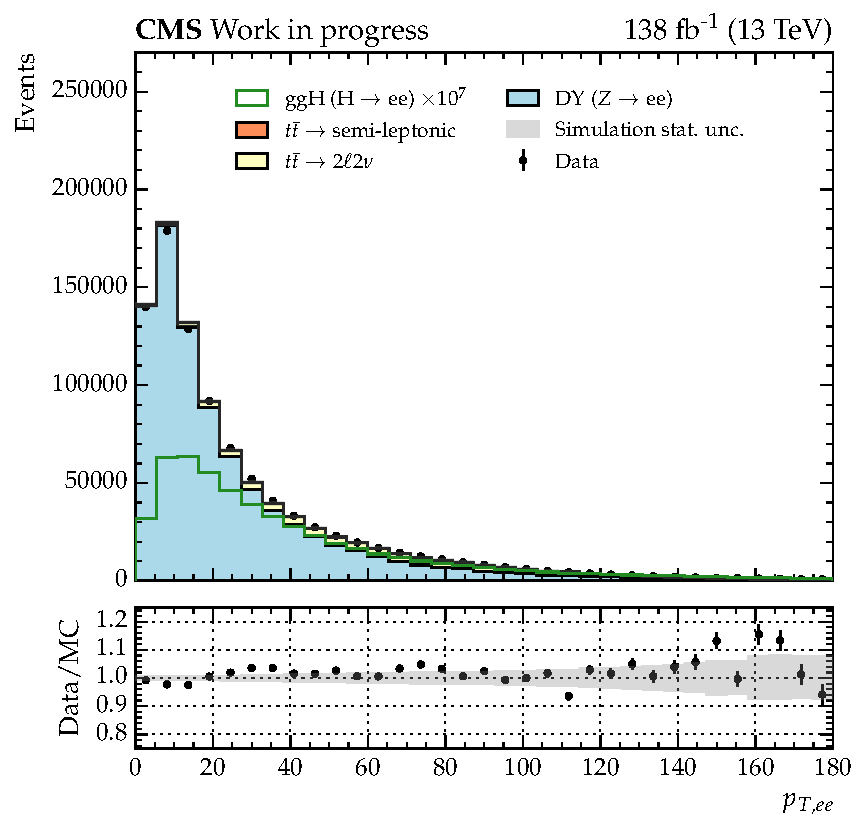
\includegraphics[width =0.33\linewidth]{Figures/Hee/ggH/dataMC/ggH_BDT_pt_reweighted_dielectronPt.pdf}\hfill%
%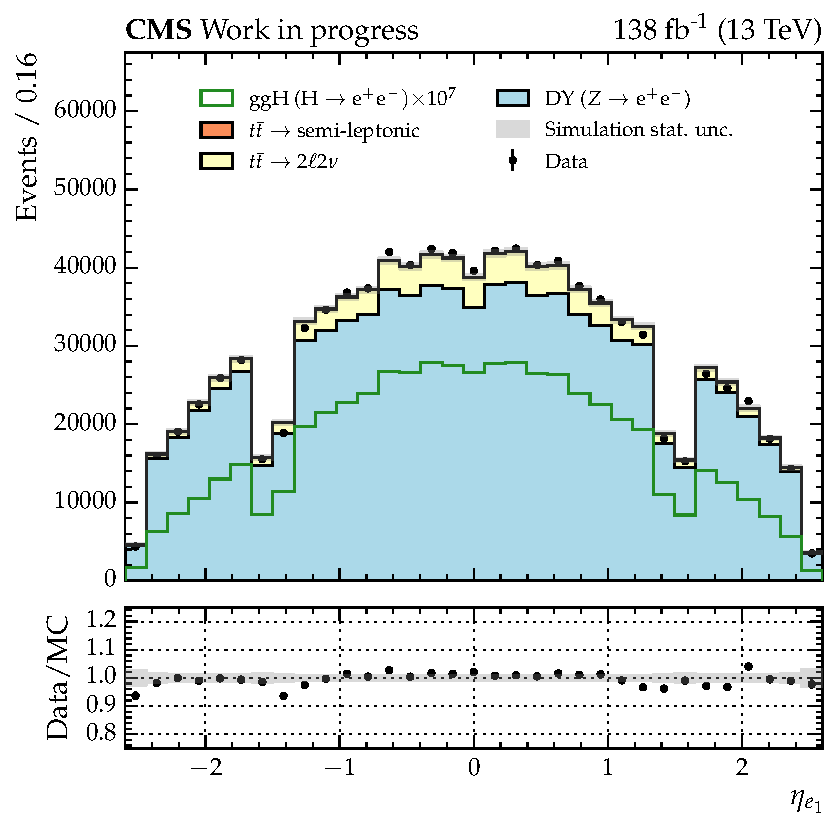
\includegraphics[width =0.32\linewidth]{Figures/Hee/ggH/dataMC/ggH_BDT_pt_reweighted_leadElectronEta.pdf}\hfill%
%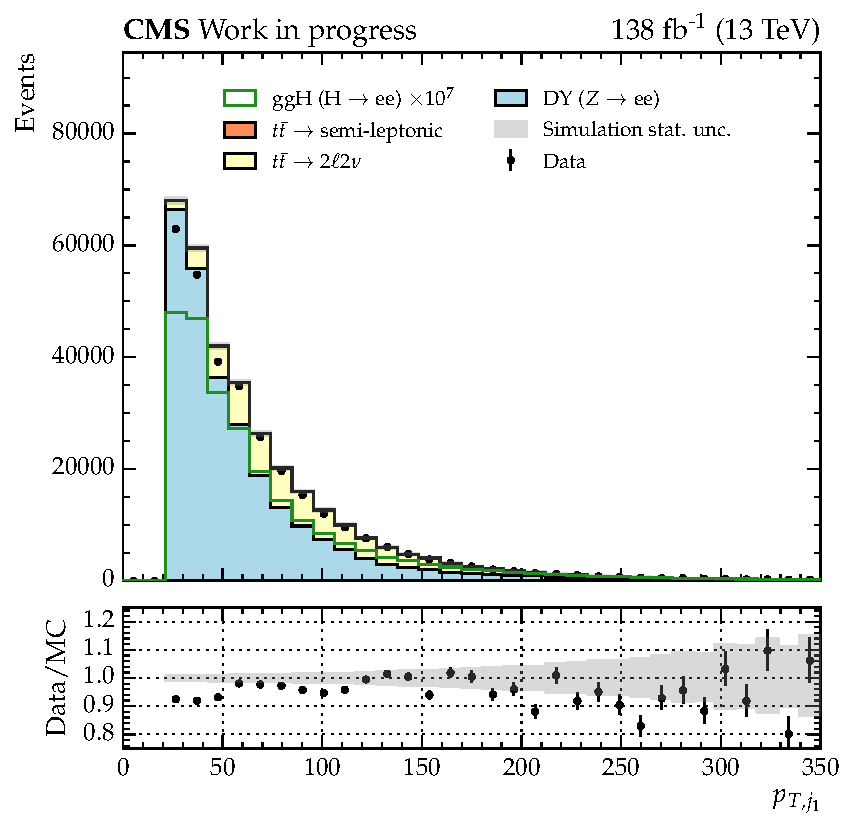
\includegraphics[width =0.33\linewidth]{Figures/Hee/ggH/dataMC/ggH_BDT_pt_reweighted_leadJetPt.pdf}\hfill%                  
%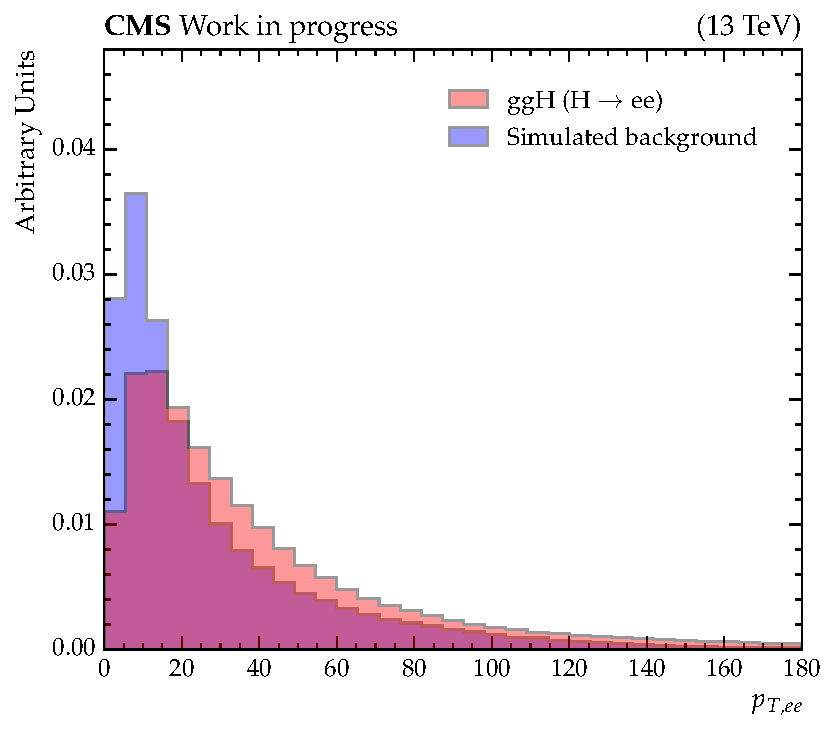
\includegraphics[width =0.33\linewidth]{Figures/Hee/ggH/normed/ggH_BDT_pt_reweighted_dielectronPt_normalised.pdf}\hfill%
%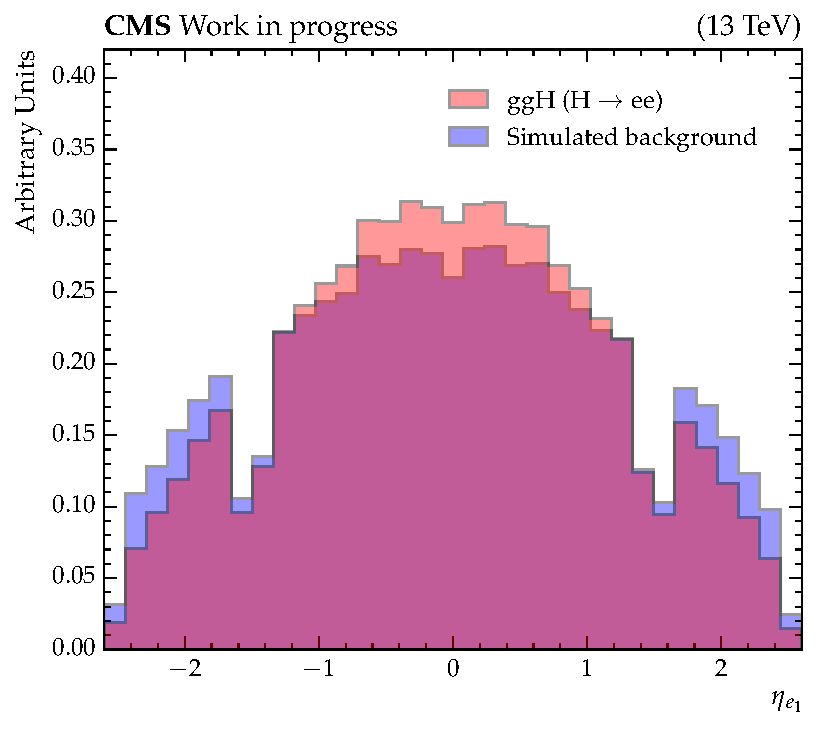
\includegraphics[width =0.32\linewidth]{Figures/Hee/ggH/normed/ggH_BDT_pt_reweighted_leadElectronEta_normalised.pdf}\hfill%
%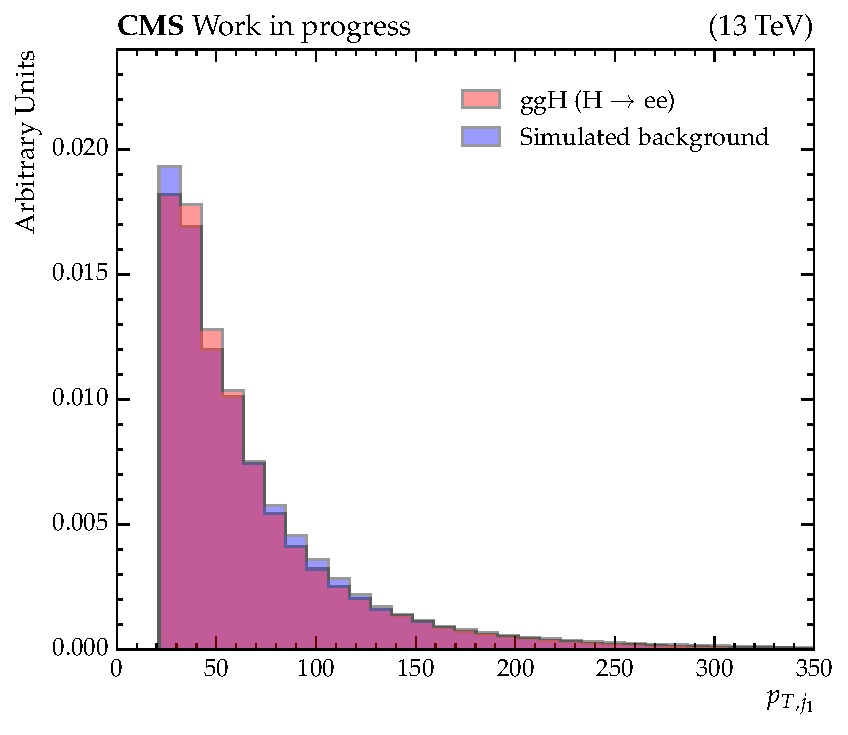
\includegraphics[width =0.33\linewidth]{Figures/Hee/ggH/normed/ggH_BDT_pt_reweighted_leadJetPt_normalised.pdf}\hfill%
%\caption[Distributions of selected input variables to the \ggH BDT.]{Distributions of selected input variables to the \ggH BDT. From left to right, these include the \pt of the dielectron object, the $\eta$ position of the leading electron, and \pt of the leading jet. Top: feature distributions for simulated background processes (bold face), stacked for comparison with data (black points). Simulated ggH signal is shown in green, with the overall normalisation scaled such that it is visible. The ratio of data to simulated background is shown in the lower panel. Reasonable agreement is observed, with respect to the statistical uncertainty (grey band). Bottom: the same input variables, normalised to unit area, with ggH signal shown in red and simulated background, integrated over each processes, shown in blue. The majority of input features show similarity between the signal and background classes, with the exception of the dielectron \pt distribution which is harder for simulated signal, and the $\eta$ position of the leading electron, which tends to be more central.}
%\label{fig:ggh_inputs}                                 
%\end{figure}   

\begin{figure}[htbp!]                                        
\centering                                                   
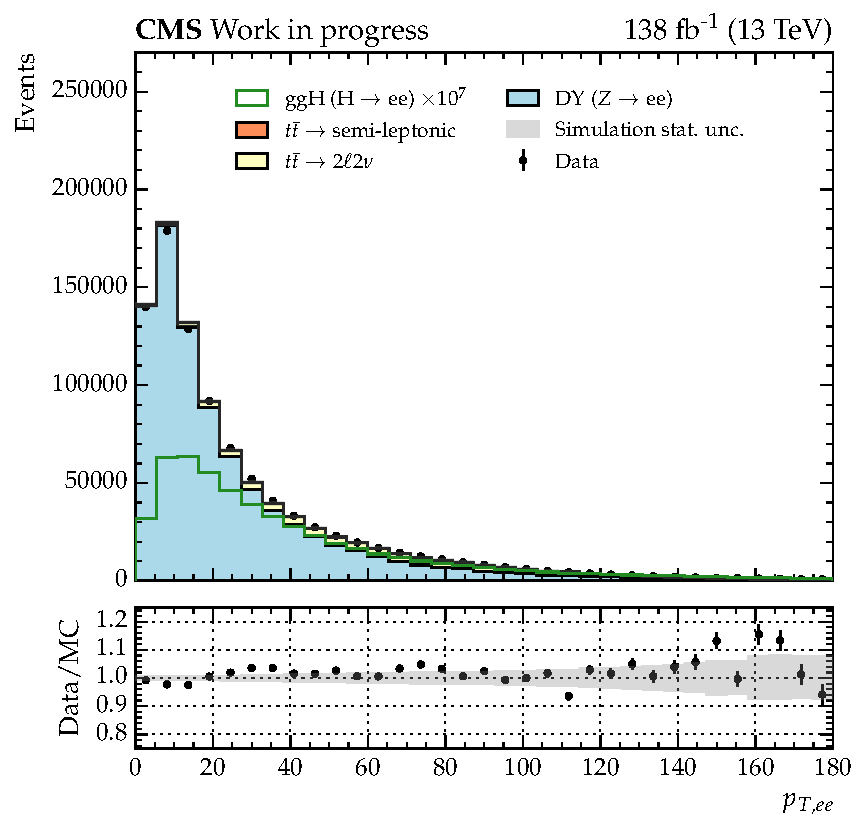
\includegraphics[width =0.407\linewidth]{Figures/Hee/ggH/dataMC/ggH_BDT_pt_reweighted_dielectronPt.pdf}\hfill%
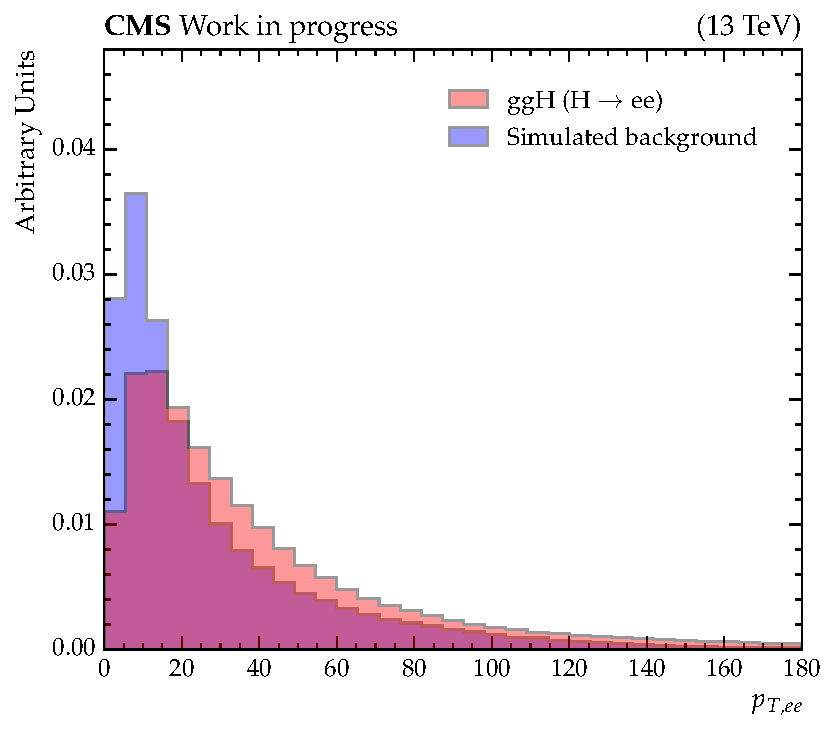
\includegraphics[width =0.45\linewidth]{Figures/Hee/ggH/normed/ggH_BDT_pt_reweighted_dielectronPt_normalised.pdf}\hfill%

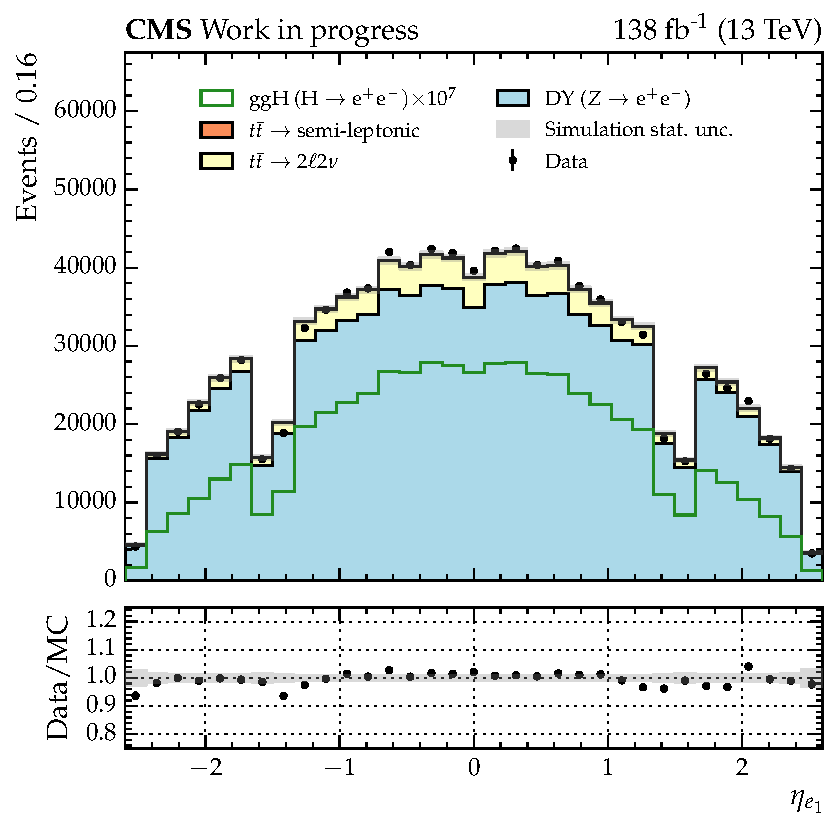
\includegraphics[width =0.395\linewidth]{Figures/Hee/ggH/dataMC/ggH_BDT_pt_reweighted_leadElectronEta.pdf}\hfill%
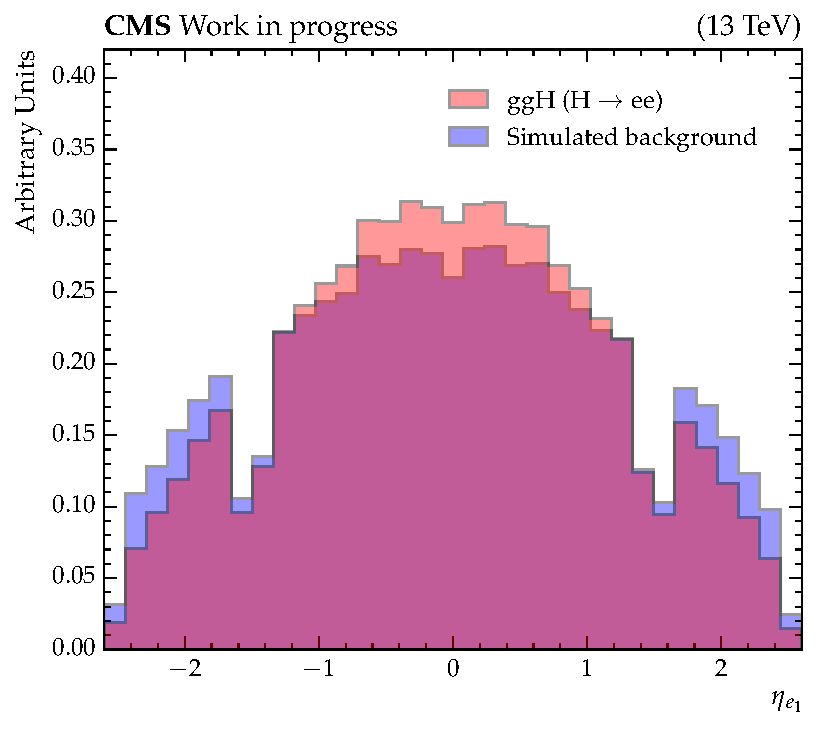
\includegraphics[trim={0mm 0mm -4mm 0mm},clip,width =0.447\linewidth]{Figures/Hee/ggH/normed/ggH_BDT_pt_reweighted_leadElectronEta_normalised.pdf}\hfill%

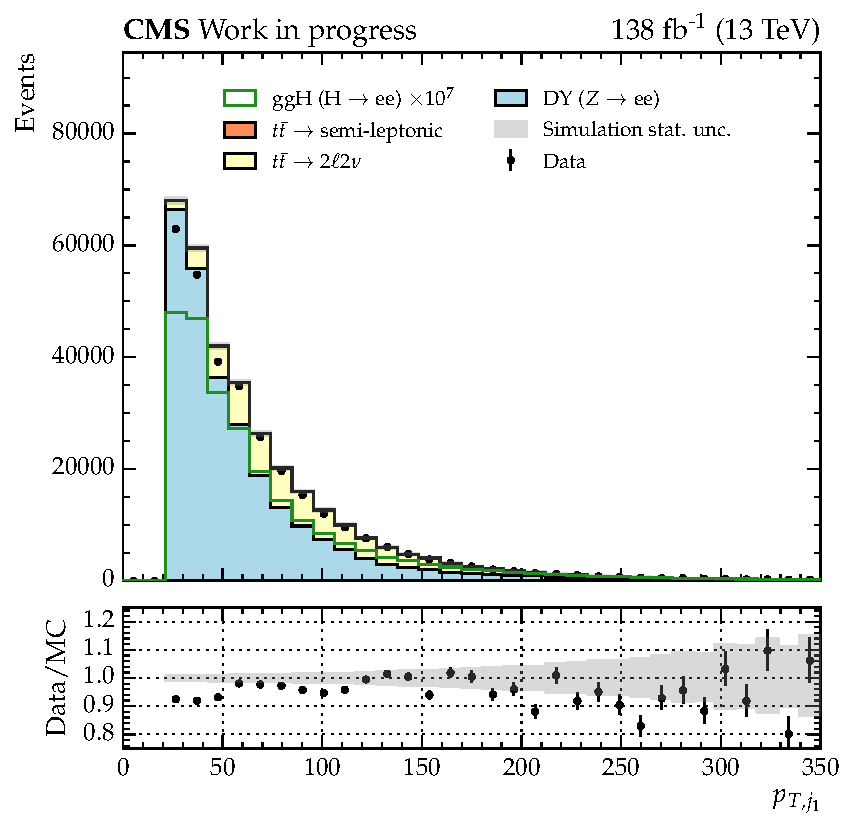
\includegraphics[width =0.403\linewidth]{Figures/Hee/ggH/dataMC/ggH_BDT_pt_reweighted_leadJetPt.pdf}\hfill%       
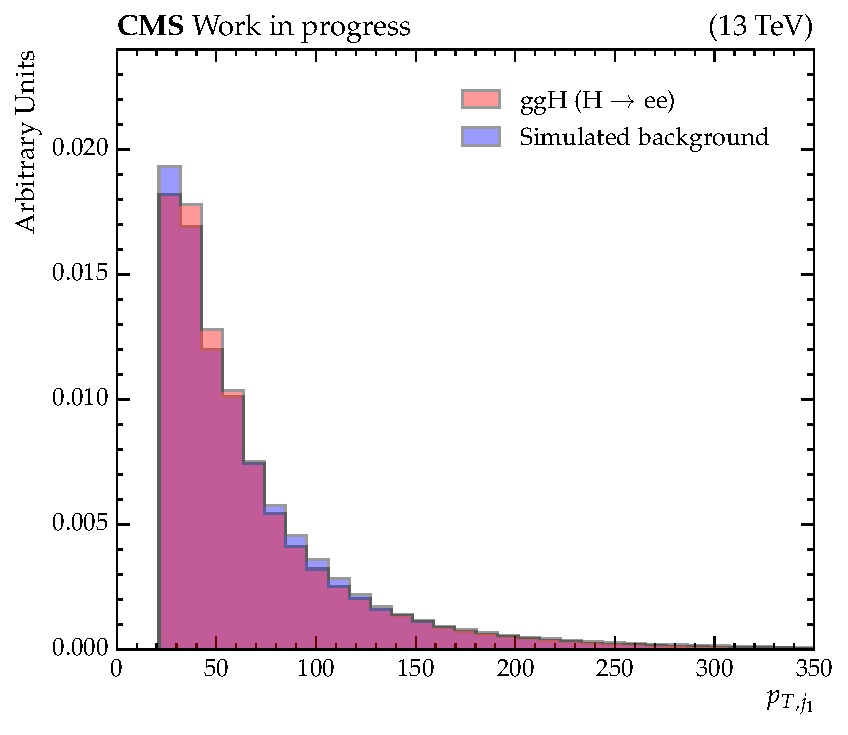
\includegraphics[width =0.454\linewidth]{Figures/Hee/ggH/normed/ggH_BDT_pt_reweighted_leadJetPt_normalised.pdf}\hfill%

\caption[Distributions of selected input variables to the \ggH BDT.]{Distributions of selected input variables to the \ggH BDT. From top to bottom row, these include the \pt of the dielectron object, the $\eta$ position of the leading electron, and \pt of the leading jet. Left: feature distributions for simulated background processes (bold face), stacked for comparison with data (black points). Simulated ggH signal is shown in green, with the overall normalisation scaled such that it is visible. The ratio of data to simulated background is shown in the lower panel. Reasonable agreement is observed, with respect to the statistical uncertainty (grey band). Right: the same input variables, normalised to unit area, with ggH signal shown in red and simulated background, integrated over each processes, shown in blue. The majority of input features show similarity between the signal and background classes, with the exception of the dielectron \pt distribution which is harder for simulated signal, and the $\eta$ position of the leading electron, which tends to be more central.}
\label{fig:ggh_inputs}                                 
\end{figure}   




\subsection{Training and optimisation}

To train the ggH BDT,  simulated \ggH events from all years passing the basic preselection are used.
Simulated background events include Drell-Yan processes which account for approximately 92\% of all background events passing preselection, alongside smaller contributions from \ttbar decays.
For both signal and background, events are weighted initially in accordance with their SM production cross section. 
The full sample of events are divided randomly into a training set, which comprises 70\% of the original sample used to train the BDT, and a testing set, which contains the remaining 30\% of events withheld to evaluate the performance of the final model. Separating the data in this way ensures that any predictions made on the test set remain unbiased to events used in the classifier training and optimisation processes, as discussed in Section~\ref{subsec:ML_model_training}.

%The BDT is implemented with using the XGBoost~\cite{xgboost} python library. The loss function, which quantifies the model performance during training, is chosen as the binary logarithmic loss, sometimes referred to as the binary cross-entropy. The cross-entropy increases as the predicted probability diverges from the true class label, resulting in heavier penalisation for models that predict class probabilities far from their true values. It is checked that alternative loss functions do not improve the classifier performance.

The BDT is implemented using the XGBoost~\cite{xgboost} python library. The implementation has multiple hyperparameters that may be tuned to improve both performance and convergence time during training. For the \ggH BDT, the main hyperparameters that govern the model complexity are optimised, including the learning rate and maximum depth of ensembled learners. Larger values of the learning rate result in quicker descent of the loss manifold, but produce models that may never converge to the global minimum. The maximum depth refers to the number of successive splits permitted for all decision trees in the ensemble. Increasing the tree depth allows the algorithm to learn a more complex function of the input feature set, which may offer increased separation power. However, increasing the depth arbitrarily may result in overfitting to statistical fluctuations in the training set. 

Since the underlying function mapping hyperparameters to performance is unknown, gradient-based methods cannot be used to find optimal configurations. 
Therefore, this analysis uses a 3-fold cross-validation technique~\cite{patternRecognitionAndML} to draw conclusions on the best model hyperparameters. This is a derivative-free method where each configuration is sampled exhaustively from a grid of all possibilities. A typical $k$-fold cross validation strategy partitions the training set into $k$ intervals, or ``folds".
The model is trained on all but one of the folds, with the remaining fold used to quantify the model performance. The process is then repeated, with a different fold being held for testing purposes and the remaining used for training. The final performance of the model is quantified by averaging the performance over all $k$ trainings. The hyperparameter search space considered for all BDTs trained in this search is given Table~\ref{tab:bdt_hps}.
\begin{table}[htbp!]
\centering
\caption[The hyperparameter search space for the BDTs used in the categorisation of \Hee events]{The hyperparameter search space for both the \ggH and VBF BDT. The final choice of parameters are chosen to maximise the model performance on a withheld validation set. The performance is largely similar across the possible hyperparameter configurations; hence the nominal values, highlighted in bold font, are used in the final models. 
}
\label{tab:bdt_hps}
\begin{tabular}{l|l}
\hline
Model hyperparameter    & Search space \\ \hline 
Learning rate & 0.01, 0.05, 0.1, \textbf{0.3}       \\
maximum tree depth & 3, 4, 5, \textbf{6}, 7, 8, 9, 10\\
regularisation coefficient ($\gamma$) & \textbf{0}--5 \\
events subsample for learners & 0.5, 0.8, \textbf{1.0} \\
number of learners & \textbf{100}, 200, 300, 400, 500 \\ 
\hline
\end{tabular}                  
\end{table}  

Another parameter that can be changed is the relative weight of the signal and background samples. With the default sample weights, which correspond to the expected number of events, the two classes are extremely imbalanced, resulting in the classifier predicting the background class for almost all events. To mitigate this, the BDT is trained in a scenario where the signal event weights are increased by a uniform factor such that the total sum of weights for signal and background processes is equal. This serves purely as a technical change to the training, designed to improve the learning outcomes of the classifier --- when evaluating the performance, the nominal weights are used. The reweighting forces the algorithm to consider each class as equally important and results in dramatically improved performance. In addition, given that the analysis sensitivity depends on the dielectron mass resolution, a second reweighting is applied to \ggH events during training to make the classifier aware of this fact. Events are weighted by 1/$\sigma(m_{ee})$, where $\sigma(m_{ee})$ is the per-event mass resolution. This strategy is preferred to simply adding $\sigma(m_{ee})$ as an input feature, since this distribution itself holds little separation power between signal and background processes.

Finally, since the dataset analysed is composed of three individual years of data taking, an alternative strategy where a single classifier is trained for each year independently is explored. This strategy could allow the classifier to take into account any per-year differences between simulated samples. However, splitting the training data more finely reduces the size of the dataset available to learn from, potentially worsening the overall performances. Two studies are performed to look for possible improvement by training independently: firstly, it is verified that including a quantity encoding the year of simulation to the input feature set does not add any discrimination power. Secondly, it is confirmed that the performance when training three separate classifiers is consistent between years. Since the results of these studies indicate little difference between simulation in each year, the classifier is trained on the combination of all simulated samples.

\subsection{Performance evaluation} 

The performance of the classifier is evaluated using the area under the ROC curve. The curve is generated by placing sequentially tighter selection on the ggH BDT output score, which is shown for both data and simulation in Figure~\ref{fig:hee_ggh_out_score_and_rocs} (left), and computing the associated true and false positive rates.
The output score distributions for ggH signal and simulated background are not well separated, which is expected from the similarity of the event kinematics.
This is reflected in the ROC curve, shown in Figure~\ref{fig:hee_ggh_out_score_and_rocs} (right), where the associated AUC score is relatively small, evaluating on the test set to 0.675.
The metric is also computed on the training set and compared to confirm no significant overfitting. %0.678 on train

\begin{figure}[htbp!]
\centering
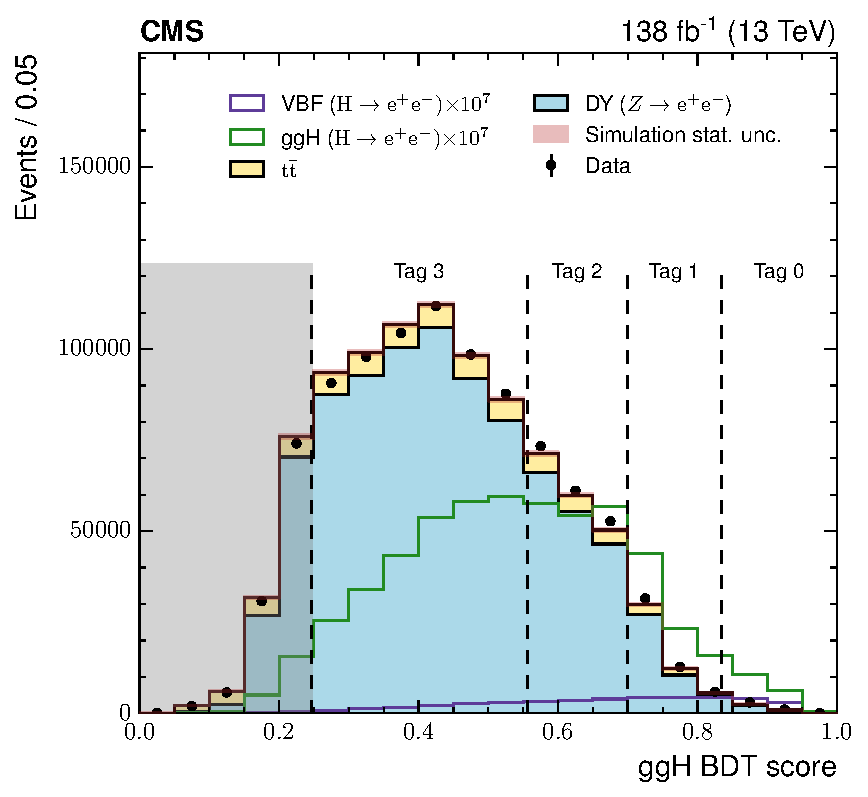
\includegraphics[width =0.47\linewidth]{Figures/Hee/ggH/dataMC/ggH_BDT_pt_reweighted_output_score_paper.pdf}\hfill%
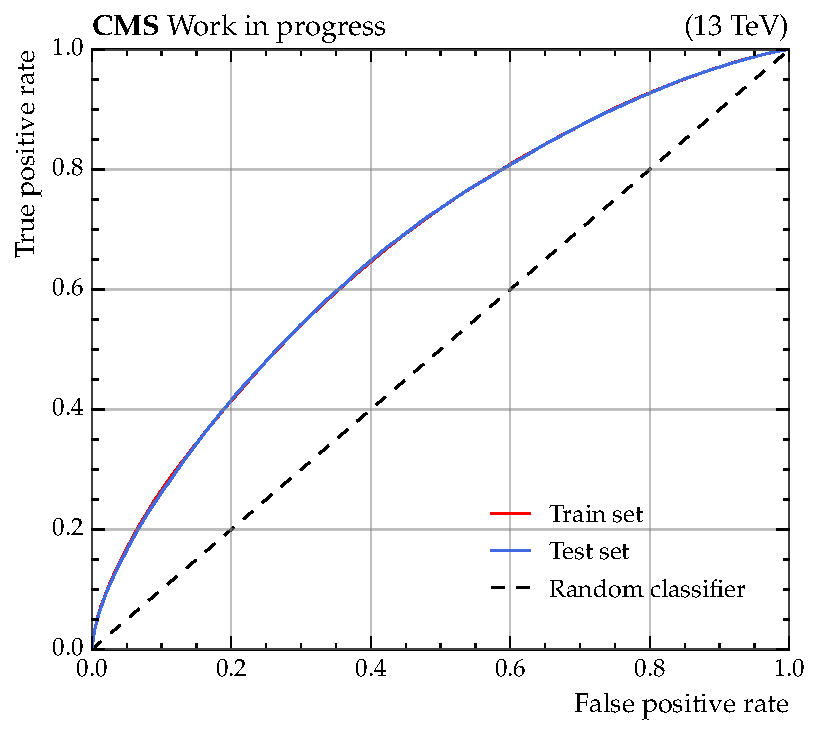
\includegraphics[width =0.48\linewidth]{Figures/Hee/ggH/dataMC/ggH_BDT_pt_reweighted_ROC_curve.pdf}\hfill%                           
\caption[The output score distribution of the \ggH BDT and associated ROC curve.]{Left: output score of the \ggH BDT for simulated signal events (green and purple histograms), background processes (bold face), and data (black markers). The distribution is similar between \ggH signal events and the Drell-Yan background, reflective of the common features between event topologies. Category boundaries targeting ggH production are denoted with dashed lines. Events with scores in the low $S/B$ grey shaded region are discarded from the analysis. Right: receiver operating characteristic curves for the \ggH BDT, evaluated on the training and testing datasets, with only \ggH events considered as signal. The area under the curves are similar for both sets, indicating no significant overtraining. The dashed line (black) provides a benchmark for a model assigning events to classes at random.}
\label{fig:hee_ggh_out_score_and_rocs}
\end{figure}

\subsection{Model interpretation}

Given that a typical gradient boosted decision tree may ensemble thousands of individual learners, each with their own set of decision nodes, it is often difficult to explain how a model arrives at a prediction. Therefore, in order to improve the so-called \textit{explainability} of the \ggH BDT, additional studies are performed to understand how each input feature is connected to the overall prediction.

Firstly, in order to understand how the \ggH BDT score is correlated with each input, Figure~\ref{fig:ggh_sig_evo} shows, for simulated \ggH signal events, the distribution of selected features as a function of the BDT output score. Red and orange colours indicate events occupying a lower BDT score interval, associated with background-like predictions, while blue and green colours correspond to signal-like events.
The BDT assigns high scores to centrally produced electrons forming a high $p_{T,ee}$ pair, features which are characteristic of the \ggH event topology.
In addition, a significant fraction of events (with two or more jets) receiving a high BDT score are characterised by a large $\Delta R$ separation between the dijet system the closest electron in the dielectron pair.
The classifier is also aware of the dielectron mass resolution, placing events with 
smaller $\sigma(m_{ee})$ at higher scores, as seen in Figure~\ref{fig:ggh_mee_and_njet_evo} (left). This effect is partially generated by the reweighting of signal events applied in training by 1/$\sigma(m_{ee})$.
Lastly, it is checked that the classifier cannot infer the value of the Higgs boson mass from the set of input features, which leads to undesirable sculpting of the \mee distribution. To illustrate this check, Figure~\ref{fig:ggh_mee_and_njet_evo} (centre) shows the \mee spectrum for simulated background events as a function of the BDT output score. The distribution remains smoothly falling in each BDT score interval, and thus is highly uncorrelated with the dielectron mass.

\begin{figure}[htbp!] 
\centering
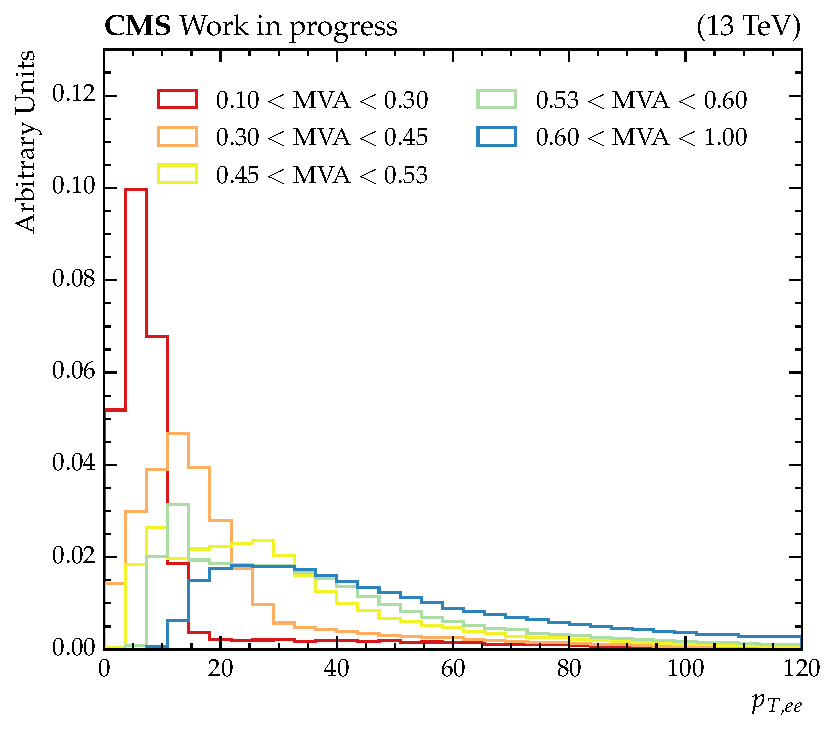
\includegraphics[width =0.333\linewidth]{Figures/Hee/ggH/featureEvo/ggH_BDT_pt_reweighted_dielectronPt.pdf}\hfill%
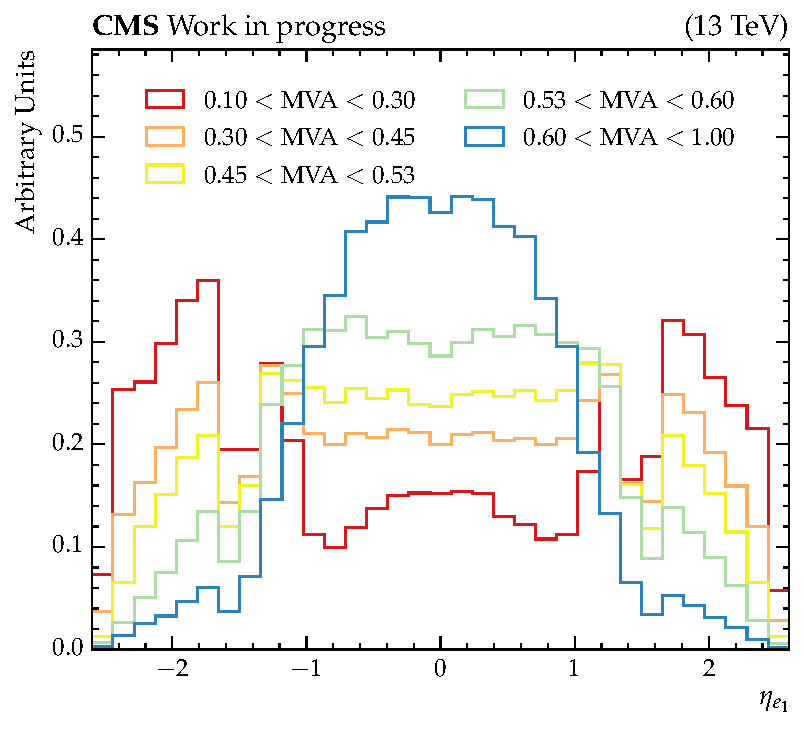
\includegraphics[width =0.32\linewidth]{Figures/Hee/ggH/featureEvo/ggH_BDT_pt_reweighted_leadElectronEta.pdf}\hfill%
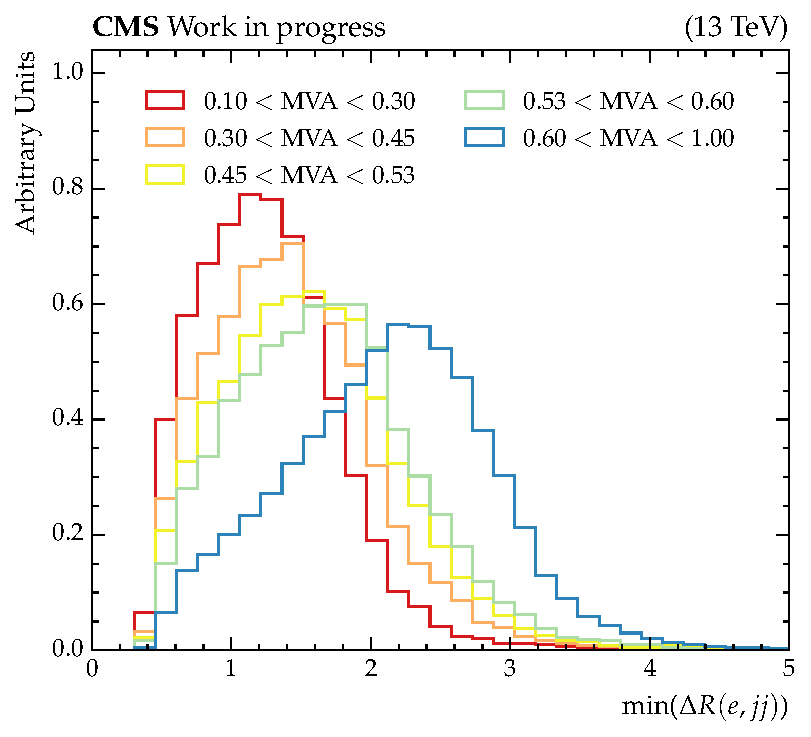
\includegraphics[width =0.32\linewidth]{Figures/Hee/ggH/featureEvo/ggH_BDT_pt_reweighted_dijetMinDRJetEle.pdf}\hfill%

\caption[Distributions of selected inputs to the \ggH BDT, as a function of BDT output score.]{Distributions for selected input variables to the \ggH BDT for simulated \ggH signal events, as a function of the \ggH BDT output score. From left to right, these include the dielectron \pt distribution, the $\eta$ position for the leading electron, and the smallest $\Delta R$ between a single electron in the dielectron pair and the dijet system. Each histogram is normalised to unit area. Blue and green colours indicate signal-like predictions, which are characterised by an electron pair with high \pt, produced centrally in the detector. Events with two jets are also assigned high scores if the dijet pair is well separated in $R$ from the closest electron in the dielectron object.}
\label{fig:ggh_sig_evo}
\end{figure}

\begin{figure}[htbp!] 
\centering 
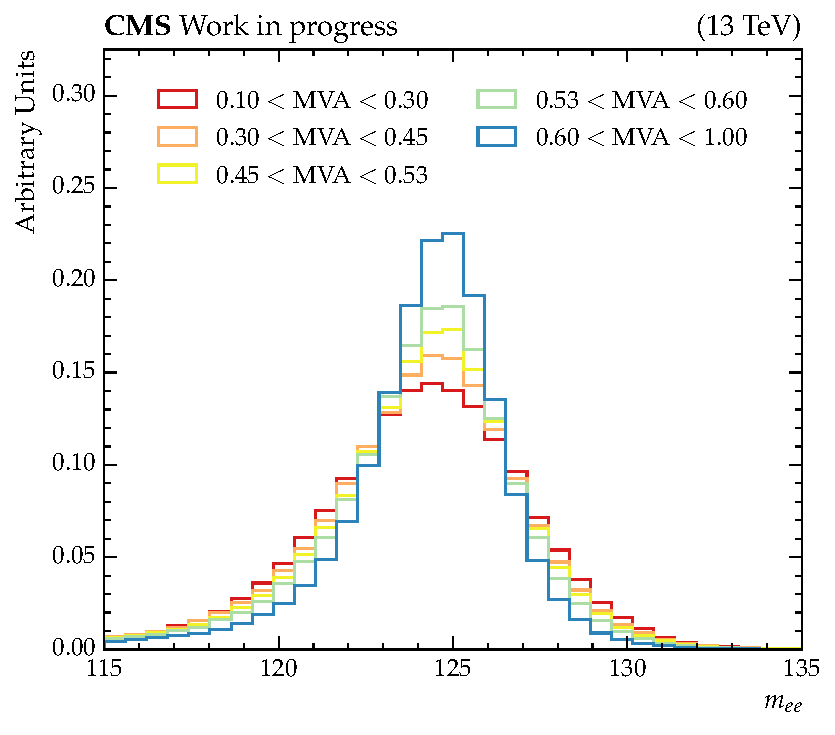
\includegraphics[width =0.33\linewidth]{Figures/Hee/ggH/featureEvo/ggH_BDT_pt_reweighted_dielectronMass.pdf}
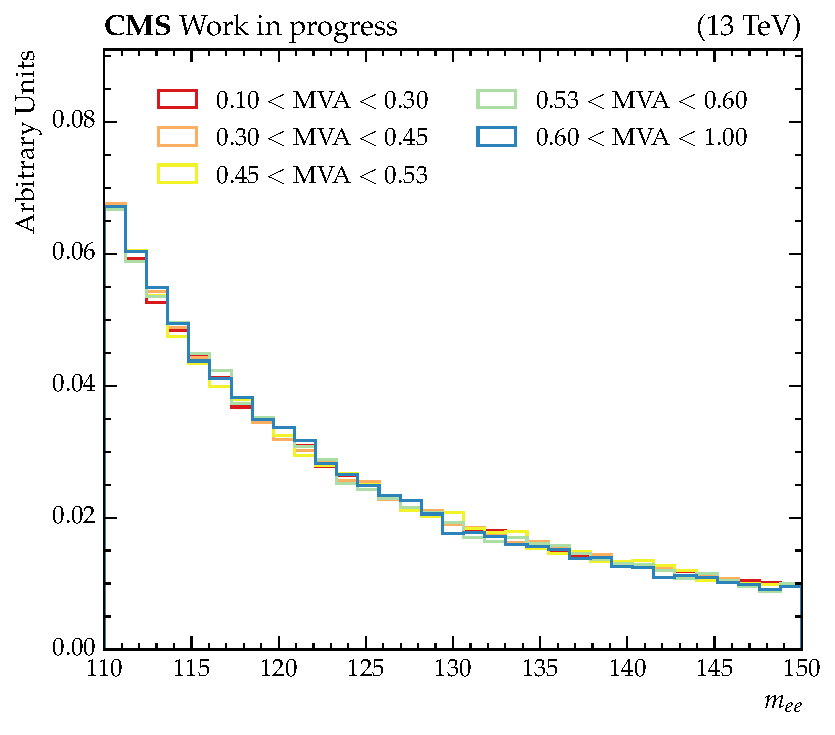
\includegraphics[width =0.33\linewidth]{Figures/Hee/ggH/featureEvo/ggH_BDT_pt_reweighted_dielectronMass_bkg.pdf}\hfill
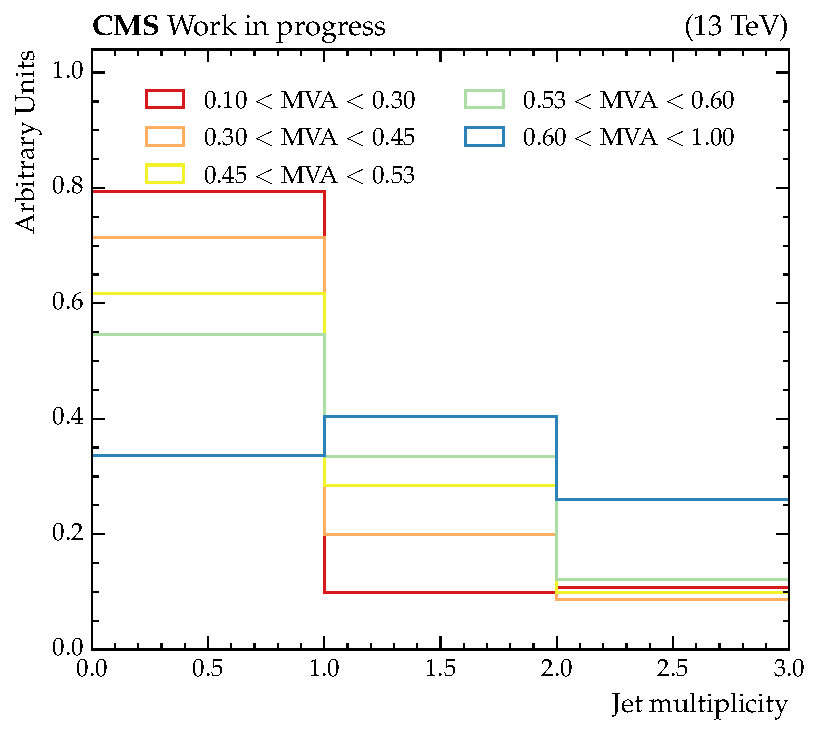
\includegraphics[width =0.32\linewidth]{Figures/Hee/ggH/featureEvo/ggH_BDT_pt_reweighted_n_jets.pdf}\hfill

\caption[The dielectron invariant mass and jet multiplicity distributions as a function of the \ggH BDT output score.]{Left: the dielectron mass distribution for simulated \ggH signal events as a function of \ggH BDT score, normalised to unit area. The classifier assigns higher scores to events with a good mass resolution. Centre: the dielectron mass distribution in simulated background events, as a function of ggH BDT score, normalised to unit area. The distribution is clearly uncorrelated with the BDT output score. Right: the jet multiplicity in various intervals of the BDT score, for simulated ggH signal events, normalised to unit area. This variable is not explicitly included in the feature set, yet the distribution evolves as a function of the output score. The BDT has therefore learned the distribution implicitly from other jet descriptions.}
\label{fig:ggh_mee_and_njet_evo}
\end{figure}

It is also useful to understand which features are good predictors for the classification task, or in other words, how important each one is when generating a prediction. The importance of each input to the \ggH BDT is ranked using Shapley values, introduced in Section~\ref{subsec:feature_selection}, with the mean of the absolute Shapley values taken as the figure of merit. Figure~\ref{fig:ggh_shap_values} shows the Shapley values for all simulated events used to train the classifier, for a selection of the most predictive features. It can be seen that events with smaller dielectron \pt values cause a large shift in predictions towards smaller (background-like) values. When evaluating the figure of merit, the dielectron \pt scores highly, as expected, alongside the leading jet QGL ID score and subleading jet \pt. 

The high importance of jet descriptions may not be forseen when considering, for example, the individual jet \pt distributions, given that these alone hold little separation power.
It is therefore hypothesised that these quantities are used by the BDT to construct some other useful feature. For example, the jet multiplicity could be inferred from the set of default values for jet \pt when a jet is not present, which are set far from the nominal range. To verify this, it is checked that the jet multiplicity for simulated signal events changes with increasing ggH BDT score, which is confirmed in Figure~\ref{fig:ggh_mee_and_njet_evo} (right). It is also verified that adding the jet multiplicity to the set of input features brings no improvement in performance, since the classifier already has access to this information implicitly. This partly illustrates the benefit of using lower-level event information when constructing a feature set, a concept discussed in more detail in Section~\ref{subsec:vbf_lstm}.

\begin{figure}[htbp!] 
\centering 
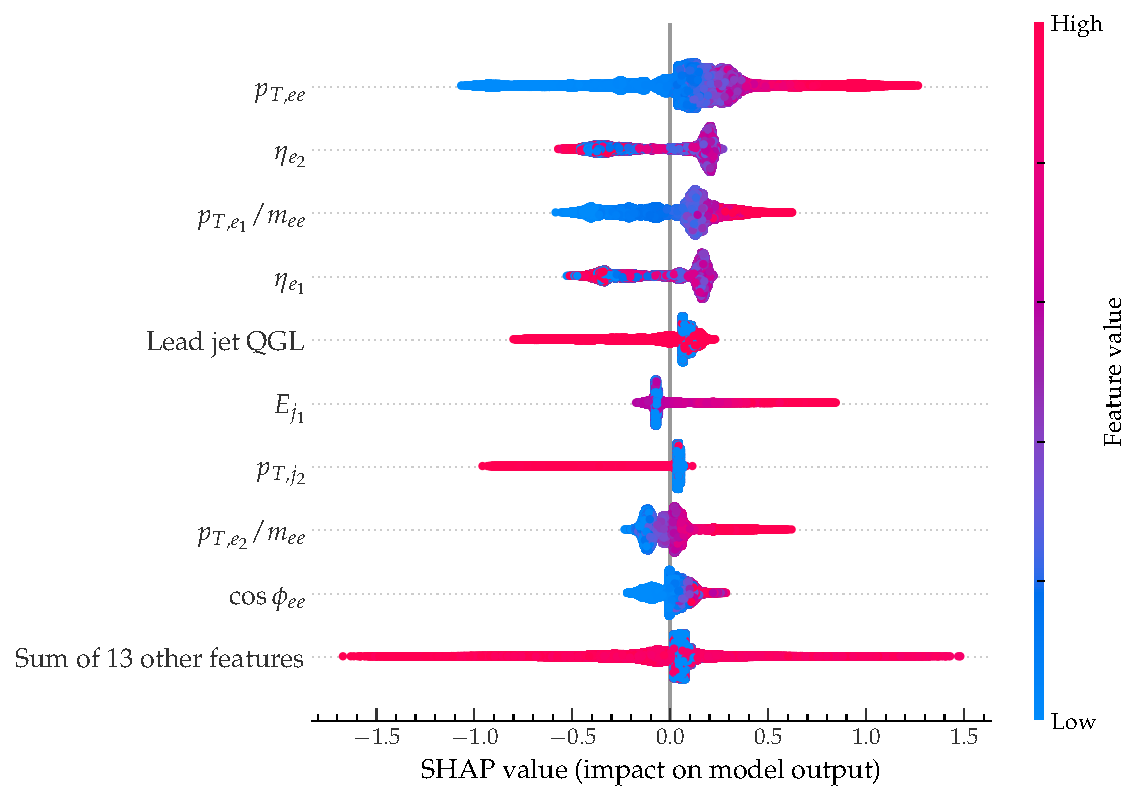
\includegraphics[width =0.8\linewidth]{Figures/Hee/ggH/featureImportances/shapley_beeswarm_ggH_BDT_featureSelection.pdf}
%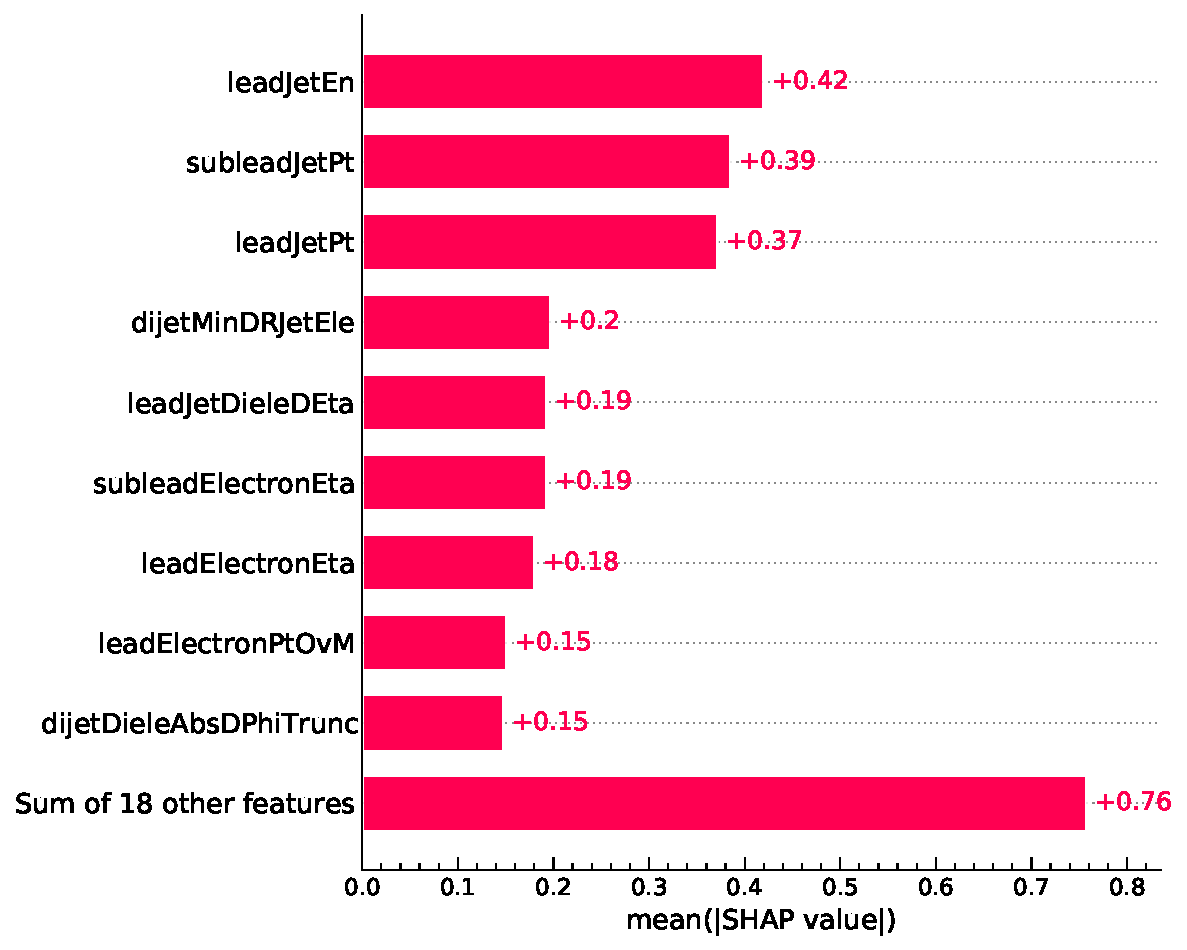
\includegraphics[width =0.8\linewidth]{Figures/Hee/ggH/featureImportances/shapley_bar_chart_ggH_BDT_pt_reweighted.pdf}
\caption[The feature importance for selected inputs to the \ggH BDT.]{The distribution of Shapley values (filled circles) for selected input features to the \ggH BDT, shown at the per-event level. Positive Shapley values indicate a preference towards signal-like predictions, while negative values are associated with background like predictions. Larger values of the input variable are coloured in red hues, while smaller values are shown by blue hues. Features are ordered by descending importance, measured by taking the mean over the magnitude of all Shapley values. Electron kinematics score highly, including the dielectron $\pt$, alongside various jet descriptions.}
\label{fig:ggh_shap_values}
\end{figure}

\subsection{Category definitions}

Categories targeting \ggH events are defined using the output score of the \ggH BDT. To construct these categories, an optimisation procedure is performed where the score distribution is divided into multiple regions, ordered by $S/B$ ratio. The Approximate Median Significance~\cite{Cowan} (AMS) is used as the figure of merit for the optimisation, defined as:

\begin{equation}
    \mathrm{AMS} = \sqrt{2\left( (S+B)\ln\left(1+\frac{S}{B}\right)-S\right)},
\end{equation}

\noindent where $S$ is the number of signal events within the window $\mH\pm\seff$, with \seff defined as the smallest interval containing 68.3\% of the signal distribution, and $B$ is the background yield. The value of $B$ is calculated by first performing an exponential fit to the \mee distribution in background, and then summing the number of events in the same integration region as the signal. Both yields are determined only for events passing the BDT selection being tested. The value of the AMS metric corresponds to the expected significance of a signal from the likelihood ratio test statistic for a simple counting experiment, neglecting the impact of systematic uncertainties. The expression reduces to the familiar $S/\sqrt{S+B}$ in the limit of small $S/B$.  

The placement of each category boundary is optimised using a random search over the parameter space. This strategy is found to be more efficient than an exhaustive grid search, particularly when the number of categories is high.
The final set of boundaries are chosen such that the AMS, combined in quadrature over categories, is maximised. 
It is found that four categories targeting \ggH events provides optimal sensitivity; no significant improvement is found when using more categories. The exact placement of each boundary is shown by the dashed lines on the output score in Figure~\ref{fig:hee_ggh_out_score_and_rocs} (left). Table~\ref{tab:hee_s_b_ams} details the expected signal and background yields, the fractional contribution from each signal process, and expected significance, for each \ggH category. Finally, the observed dielectron mass distribution in each \ggH analysis category is shown for simulated \ggH signal and background events, and data, in Figure~\ref{fig:ggh_mee_dataMC}.

\begin{table}[htb]
\caption[The number of expected \Hee signal events in each analysis category, alongside the signal resolution and expected $S/B$ ratio.]{Table showing the total expected number of signal events for \mH$=125.38$~GeV, the current best measurement of the Higgs boson mass~\cite{CMS_Hgg_Hmass}, in analysis categories targeting \ggH and VBF events, for an integrated luminosity of 138~\fbinv. The fractional contribution from each production mode to each category is also shown. The $\seff$, defined as the smallest interval containing 68.3\% of the \mee distribution, is listed for each analysis category. 
The final column shows the expected ratio of signal to signal-plus-background, S/(S+B), where S and B are the numbers of expected signal and background events in a $\pm~\seff$ window centred on $\mH$.}
\label{tab:hee_s_b_ams}
\resizebox{\columnwidth}{!}{%
\begin{tabular}{r|c|cccc|c|c|c}
\hline
Analysis category & Signal yield       & \multicolumn{4}{c|}{Production mode fractions} & $\sigma_{\mathrm{eff}}$ & Bkg per GeV & S/(S+B)               \\ \cline{3-6}
                  & ($\times 10^{-4}$) & \ggH       & VBF        & VH        & ttH      & (GeV)                   &             &                     \\ \hline
\ggH Tag 0        & 4.7                & 81\%       & 12.1\%     & 5.0\%     & 1.9\%    & 1.65                    & 250         & 7.7$\times 10^{-7}$ \\
\ggH Tag 1        & 18                 & 86.5\%     & 8.4\%      & 4.2\%     & 0.9\%    & 1.84                    & 2340        & 2.8$\times 10^{-7}$ \\
\ggH Tag 2        & 35                 & 91.7\%     & 4.8\%      & 3.1\%     & 0.5\%    & 2.02                    & 8760        & 1.4$\times 10^{-7}$ \\
\ggH Tag 3        & 61                 & 92.6\%     & 3.5\%      & 3.2\%     & 0.7\%    & 2.52                    & 30500       & 5.4$\times 10^{-8}$ \\
VBF Tag 0         & 2.2                & 19.8\%     & 80.0\%     & 0.1\%     & 0.1\%    & 2.04                    & 25.9        & 2.8$\times 10^{-6}$ \\
VBF Tag 1         & 1.7                & 40.3\%     & 58.5\%     & 0.8\%     & 0.4\%    & 2.26                    & 81.7        & 6.3$\times 10^{-7}$ \\ \hline
\end{tabular}
}
\end{table}


\begin{figure}[htbp!]
\centering
\hspace{1mm}
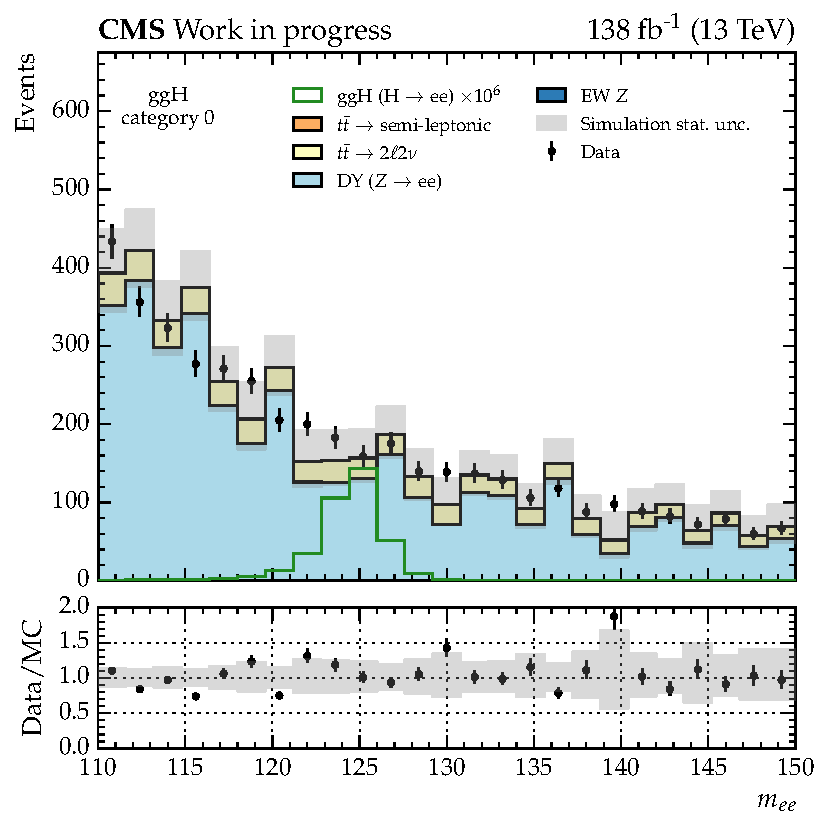
\includegraphics[width =0.465\linewidth]{Figures/Hee/ggH/MeePlots/ggH_BDT_pt_reweighted_dielectronMass_cat0.pdf}\hfill%
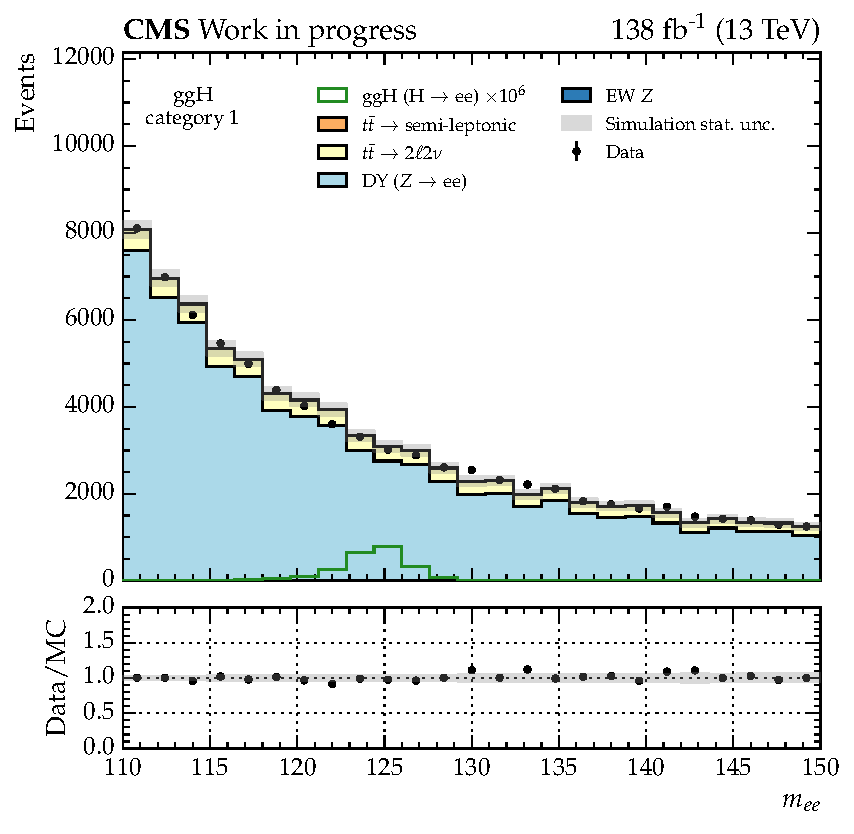
\includegraphics[width =0.48\linewidth]{Figures/Hee/ggH/MeePlots/ggH_BDT_pt_reweighted_dielectronMass_cat1.pdf}\hfill%
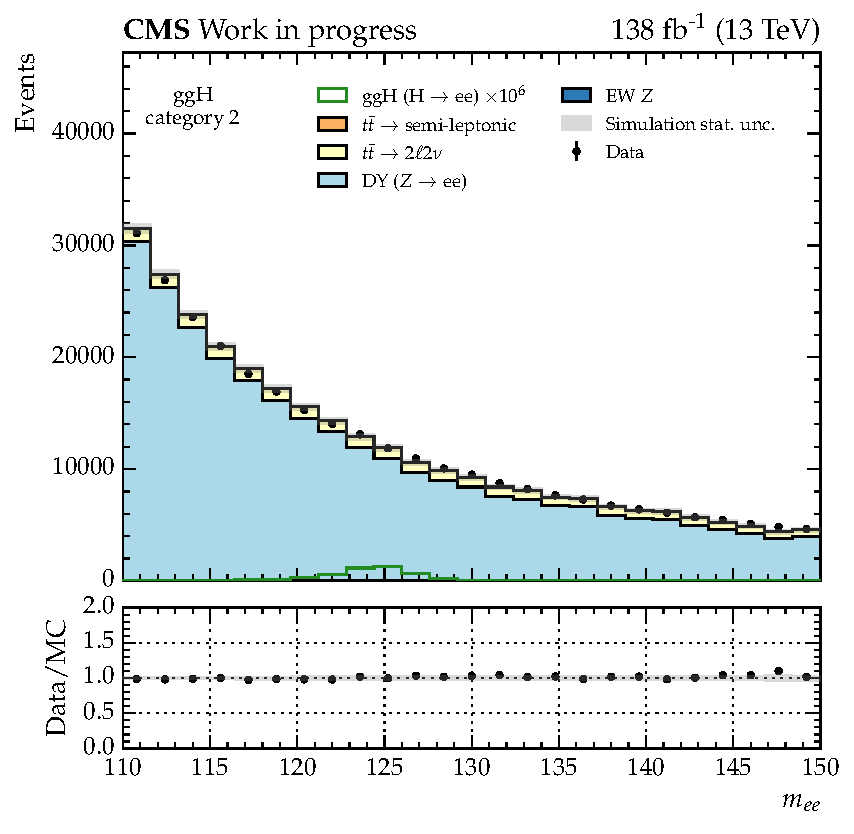
\includegraphics[width =0.48\linewidth]{Figures/Hee/ggH/MeePlots/ggH_BDT_pt_reweighted_dielectronMass_cat2.pdf}\hfill%
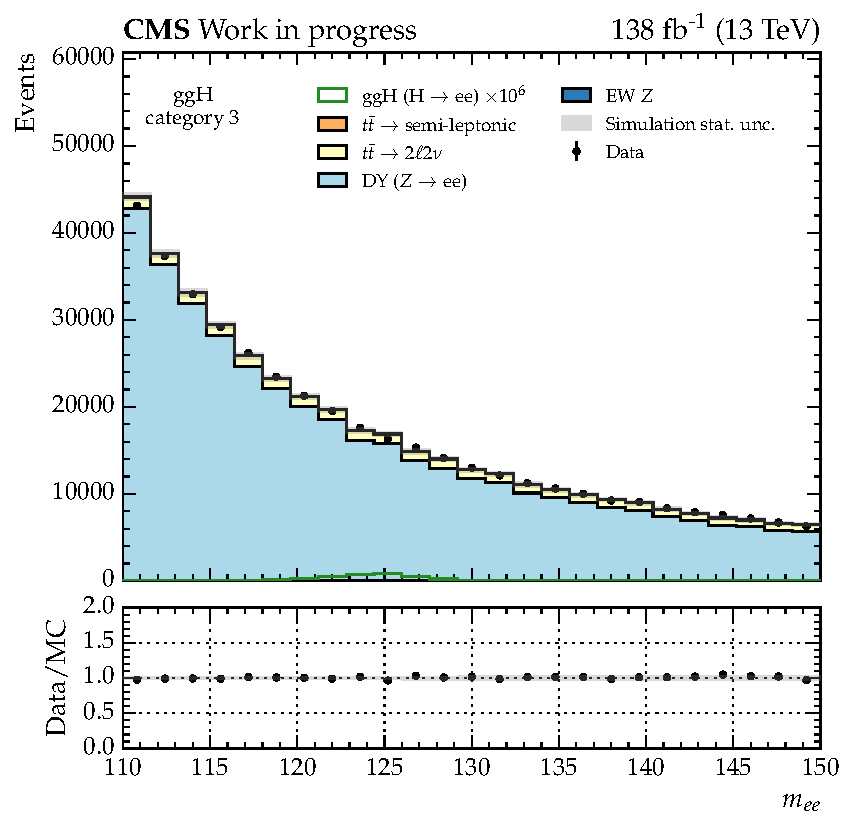
\includegraphics[width =0.48\linewidth]{Figures/Hee/ggH/MeePlots/ggH_BDT_pt_reweighted_dielectronMass_cat3.pdf}\hfill%
\caption[The dielectron invariant mass distributions for analysis categories targeting \ggH events.]{Observed \mee distributions for the analysis categories targeting \ggH events, shown for simulated background (bold face) and data (black points). The statistical uncertainty on the simulated background is shown by the grey shaded band. Simulated \ggH signal events are also shown (green), scaled such that they are visible. The ratio of data to the total simulated background is shown in the lower panels.}
\label{fig:ggh_mee_dataMC}
\end{figure} 



%%%%%%%%%%%%%%%%%%%%%%%%%%%%%%%%%%%%%%%%%%%%%%%%%%%%%%%%%%%

\section{Categories targeting VBF events}
\label{subsec:vbf_categorisation}

The nominal categorisation strategy used to target VBF events is similar to that used for \ggH. Analysis regions are defined using the output score of a BDT trained to discriminate between VBF signal and background events, referred to as the VBF BDT. Alternative categorisation strategies using deep learning techniques are also presented in Section~\ref{subsec:vbf_lstm}. 

The background composition in this channel is significantly different than for the \ggH BDT, comprising roughly equal numbers of Drell-Yan and \ttbar events. 
Additionally, electroweak $\mathrm{Z}$ boson production, where the two electrons resulting from the $\mathrm{Z}$ decay are produced in association with two quark-initiated jets, are also considered. Although these events account for less than 2\% of the total background passing VBF preselection, their kinematics and event topology are similar to the VBF signal, making them more difficult to separate compared with the dominant backgrounds. 

The VBF categories are defined firstly by applying additional requirements on top of the nominal analysis preselection, to favour events with VBF-like topology. This is referred to as the VBF preselection and comprises the following requirements:

\begin{itemize}
    \item transverse momentum of the leading (subleading) jet $> 40$ (25)~GeV, and
    \item dijet invariant mass greater than 350 GeV.
\end{itemize}

\noindent All simulated signal and background events passing the VBF preselection are used to train the VBF BDT. It is checked that including residual \ggH events that pass the VBF preselection does not improve the resulting sensitivity of the VBF analysis categories (and vice-verse when training the \ggH BDT). 

\subsection{Input features}

The set of input features provided to the VBF BDT include kinematics of the individual electrons, dielectron system, and hadronic jets. The feature set is similar to the \ggH BDT, with the exception that descriptions of a third leading jet are also included. This results in the addition of five new variables: the four vector and QGL ID score for the third leading jet. The distribution of selected input features to the VBF BDT with good prediction power are shown in Figure~\ref{fig:vbf_inputs} (left) for simulated VBF signal and background events, and data. Also shown in Figure~\ref{fig:vbf_inputs} (right) are the simulated distributions normalised to unit area, allowing for shape comparison between the signal and background events. In comparison to the \ggH BDT, many inputs display good separation power; VBF events typically include a dijet pair with high invariant mass and large opening angle in $\eta$ between the two constituent jets, features which allow for significant suppression of background events. Additionally, considerable separation of events are observed in the centrality distribution, where the VBF signal typically peaks at values close to one, while background events occupy values nearer to zero. Distributions for all inputs to the VBF BDT are provided in Appendix~\ref{app:all_input_features}.

%\begin{figure}[htbp!]                                        
%\centering                                                   
%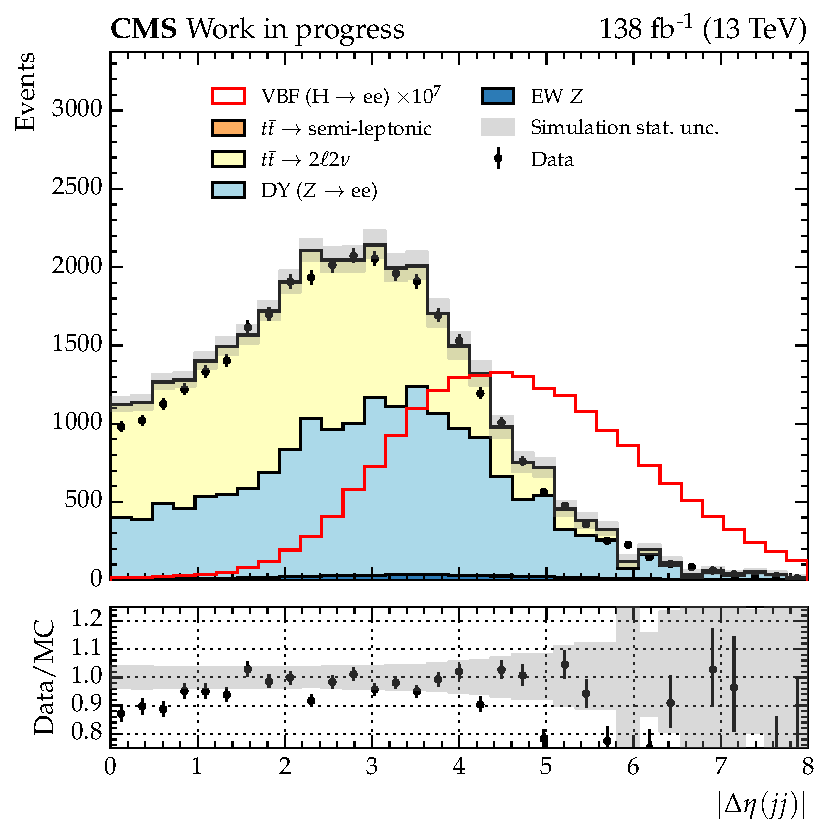
\includegraphics[width =0.33\linewidth]{Figures/Hee/VBF/dataMC/VBF_BDT_dijetAbsDEta.pdf}\hfill%
%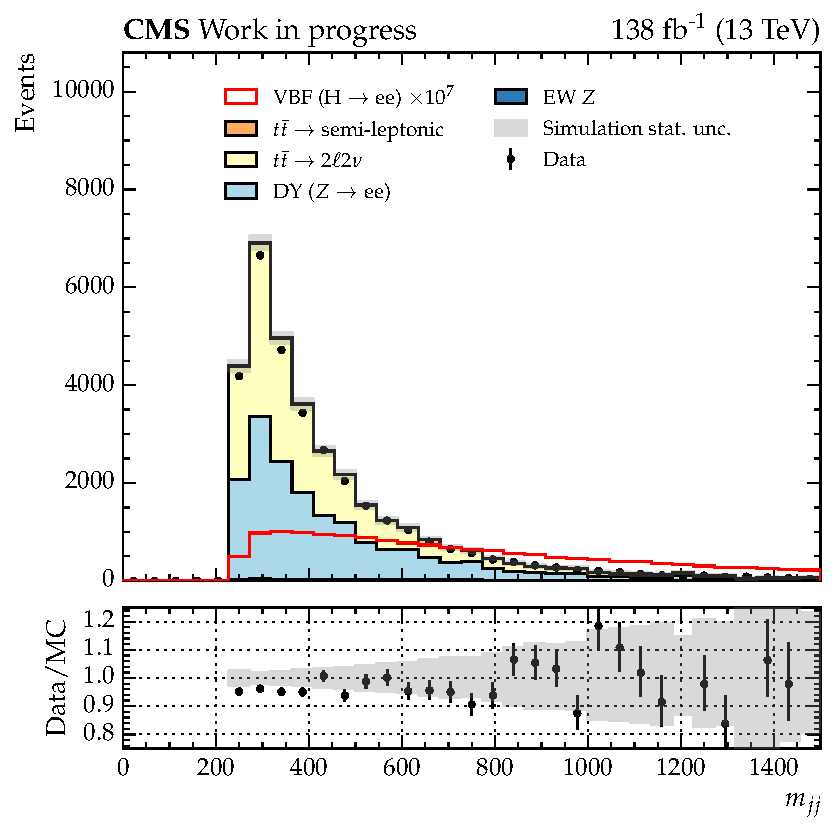
\includegraphics[width =0.33\linewidth]{Figures/Hee/VBF/dataMC/VBF_BDT_dijetMass.pdf}\hfill%
%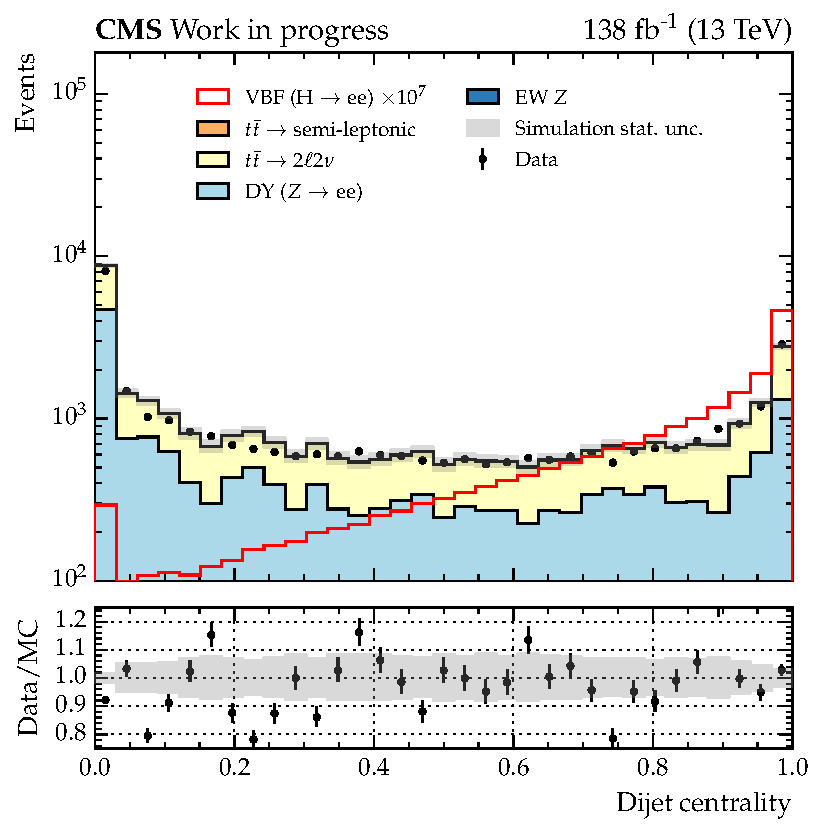
\includegraphics[width =0.33\linewidth]{Figures/Hee/VBF/dataMC/VBF_BDT_dijetCentrality.pdf}\hfill%                  
%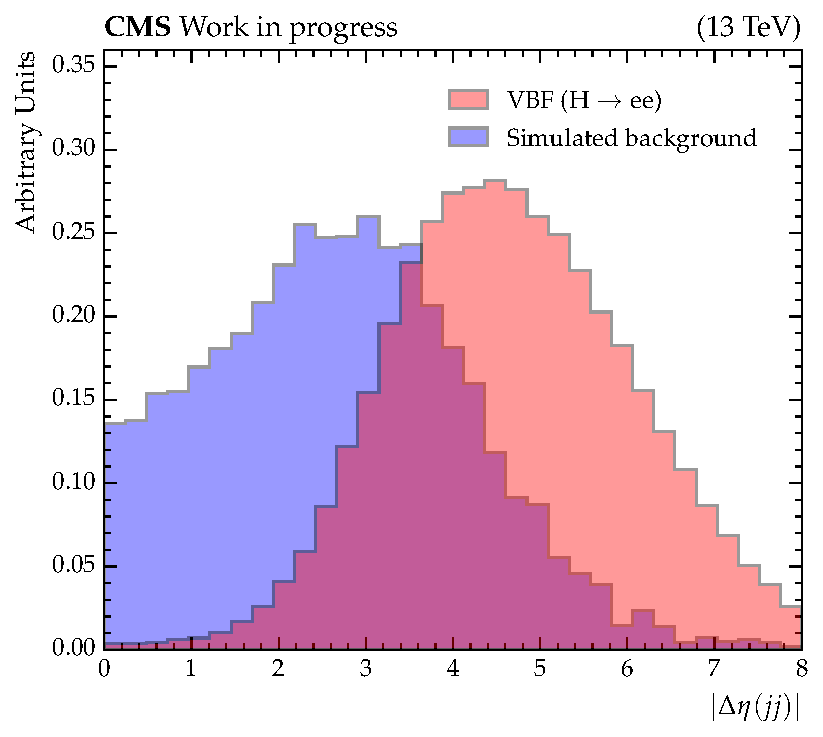
\includegraphics[width =0.33\linewidth]{Figures/Hee/VBF/normed/VBF_BDT_dijetAbsDEta_normalised.pdf}\hfill%
%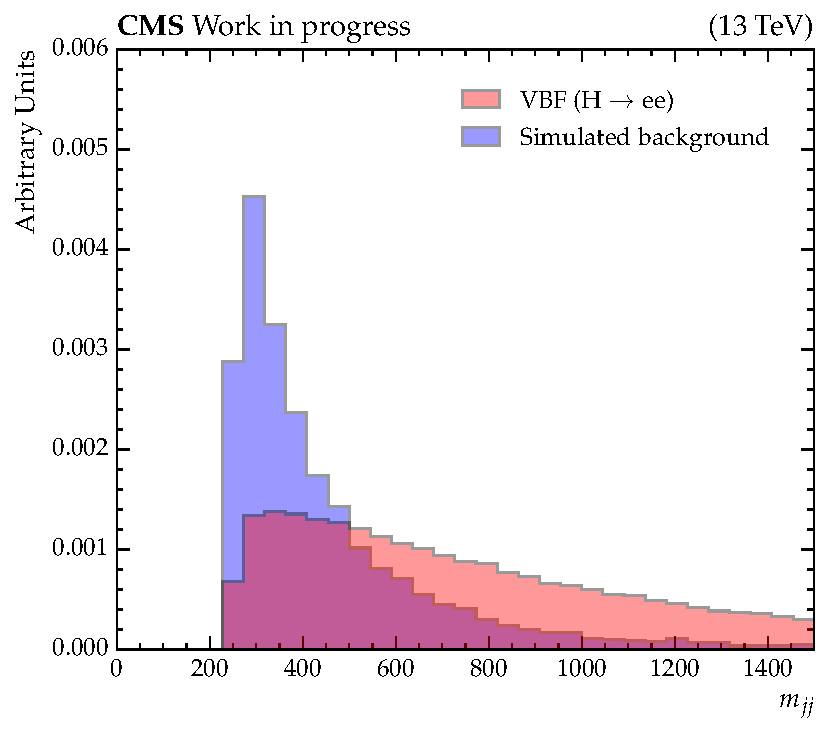
\includegraphics[width =0.33\linewidth]{Figures/Hee/VBF/normed/VBF_BDT_dijetMass_normalised.pdf}\hfill%
%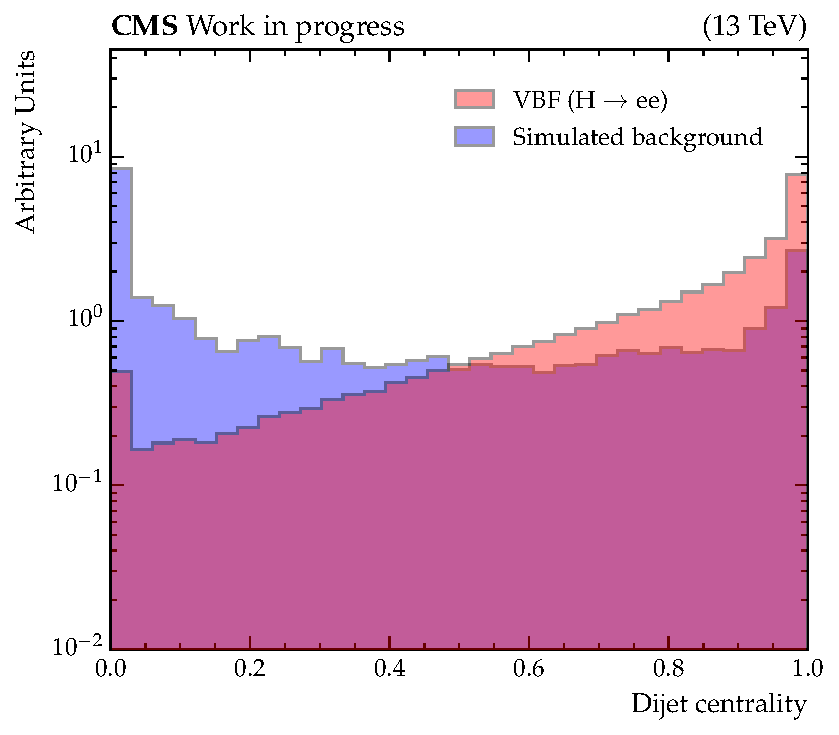
\includegraphics[width =0.33\linewidth]{Figures/Hee/VBF/normed/VBF_BDT_dijetCentrality_normalised.pdf}\hfill%

%\caption[Distributions of selected input variables to the VBF BDT.]{The distributions for selected input variables to the VBF BDT. From left to right, these include the magnitude of the difference in $\eta$ position between the leading two jets, the invariant mass of the system defined by the leading and subleading jets, and the centrality variable defined by the $\eta$ positions of the two leading jets and dielectron system. Top: feature distributions for simulated background processes (bold face), stacked for comparison with data (black points). Simulated VBF signal is also shown (red histogram), with the overall normalisation scaled such that it is visible. Reasonable agreement is observed between data and simulation, with respect to the statistical uncertainty (grey band). Bottom: the same input variables, normalised to unit area, with VBF signal shown in red, and simulated background integrated over each processes shown in blue. In general, the set of VBF input features display good separation between signal and background events.}
%\label{fig:vbf_inputs}                                 
%\end{figure}   

\begin{figure}[htbp!]                                        
\centering                                                   
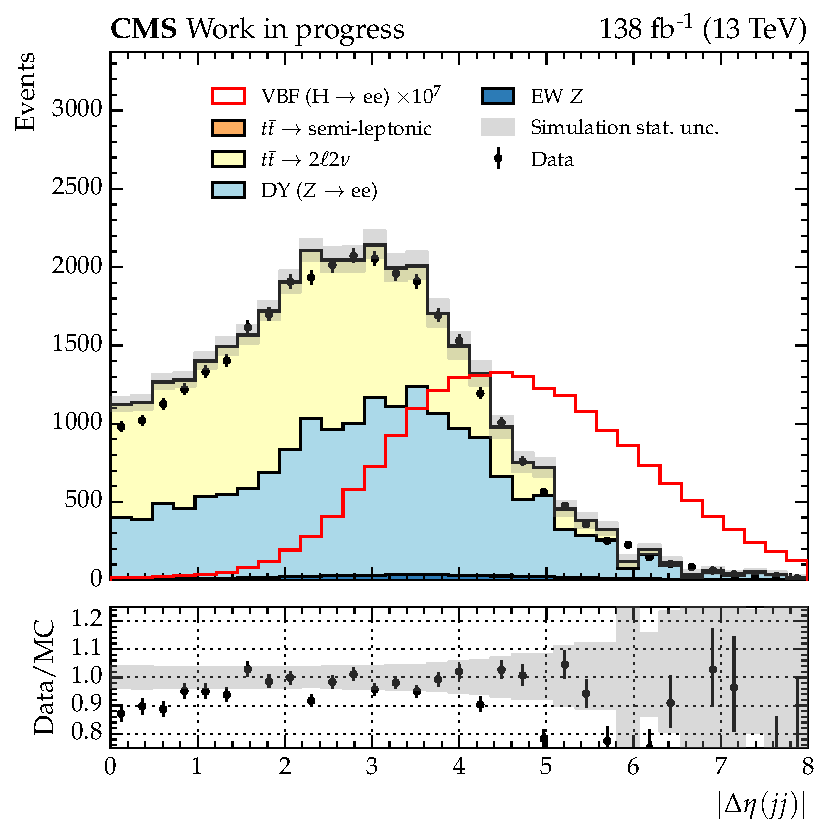
\includegraphics[width =0.4\linewidth]{Figures/Hee/VBF/dataMC/VBF_BDT_dijetAbsDEta.pdf}\hfill%
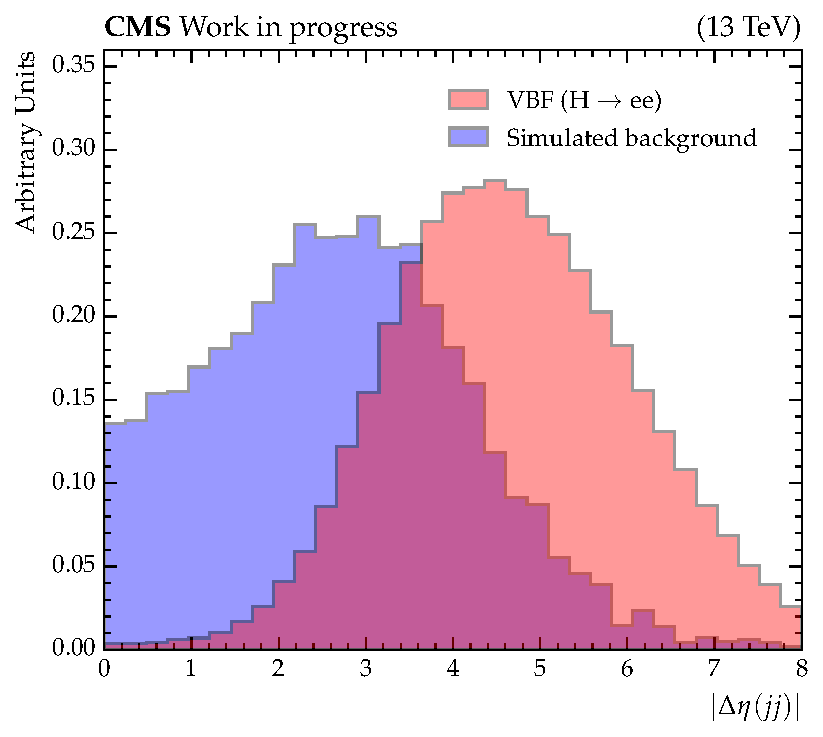
\includegraphics[width =0.45\linewidth]{Figures/Hee/VBF/normed/VBF_BDT_dijetAbsDEta_normalised.pdf}\hfill%


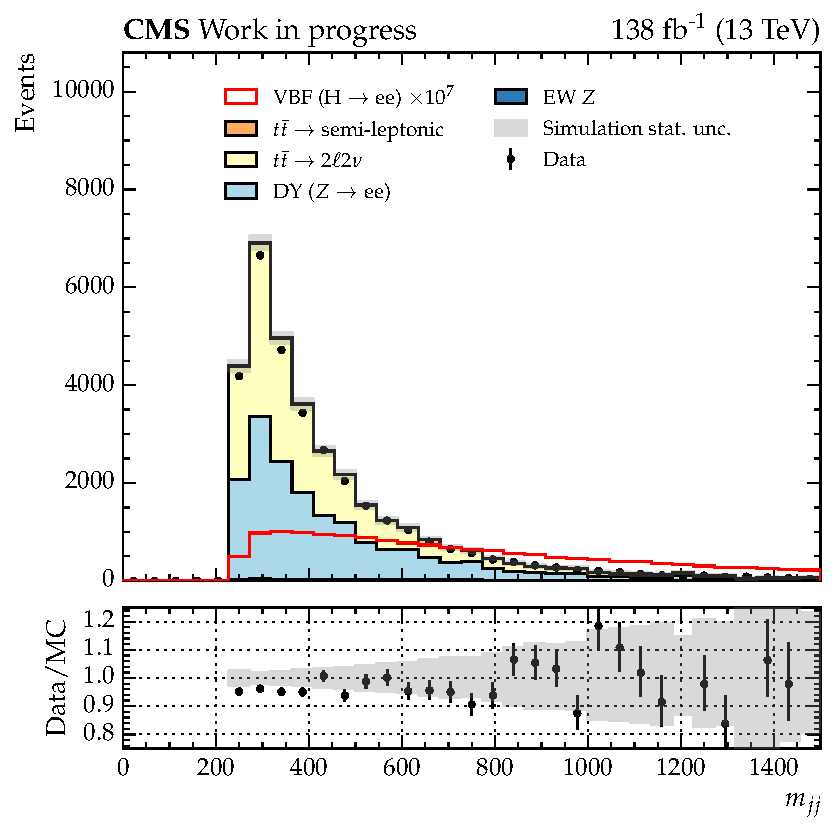
\includegraphics[width =0.405\linewidth]{Figures/Hee/VBF/dataMC/VBF_BDT_dijetMass.pdf}\hfill%
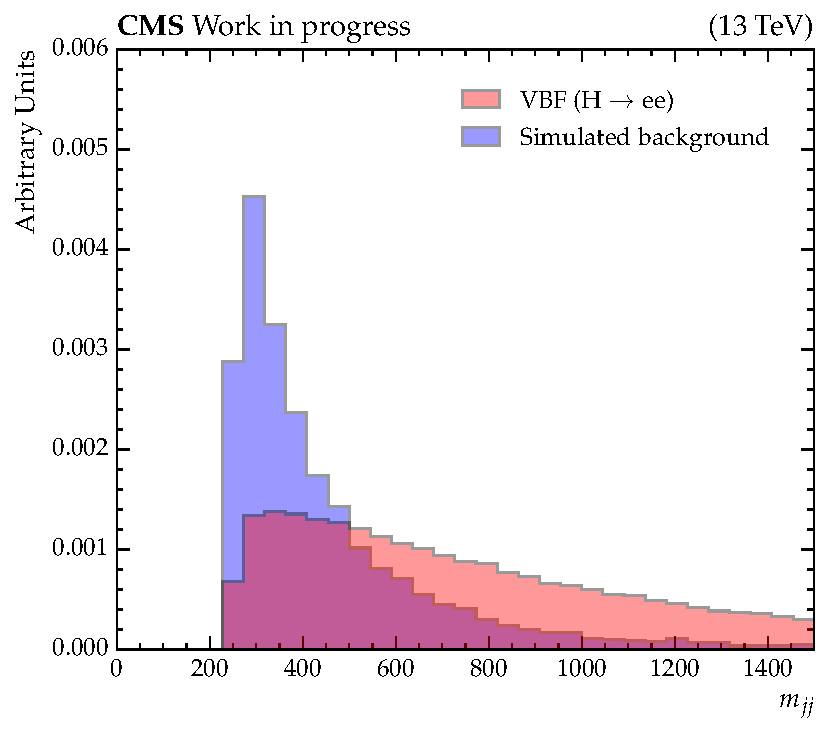
\includegraphics[width =0.45\linewidth]{Figures/Hee/VBF/normed/VBF_BDT_dijetMass_normalised.pdf}\hfill%

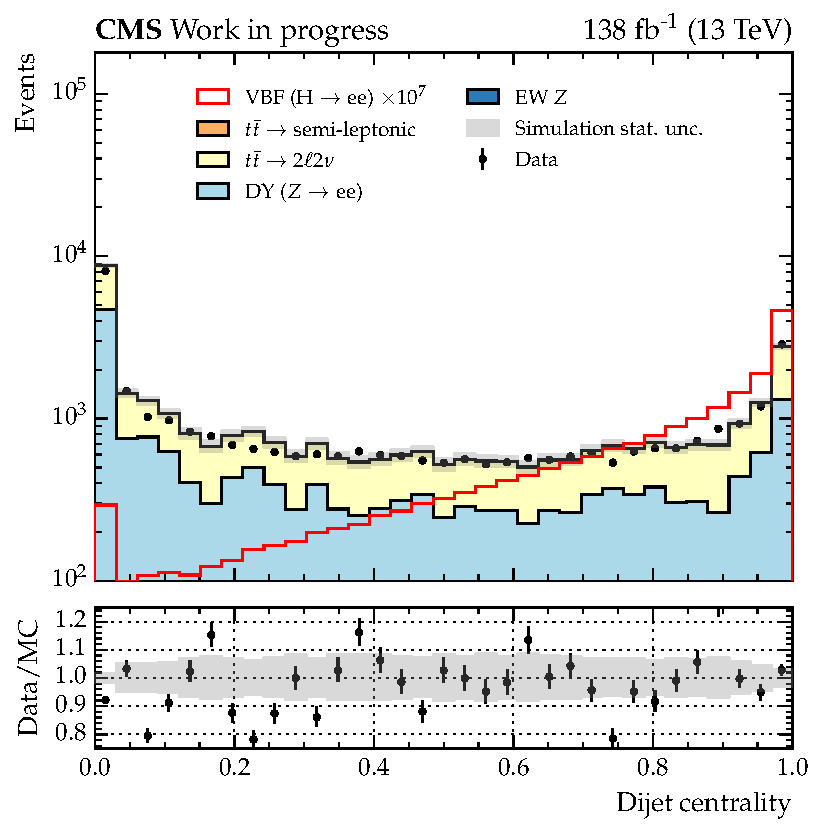
\includegraphics[trim={-5mm 0mm 0mm 0mm},clip,width =0.413\linewidth]{Figures/Hee/VBF/dataMC/VBF_BDT_dijetCentrality.pdf}\hfill%        
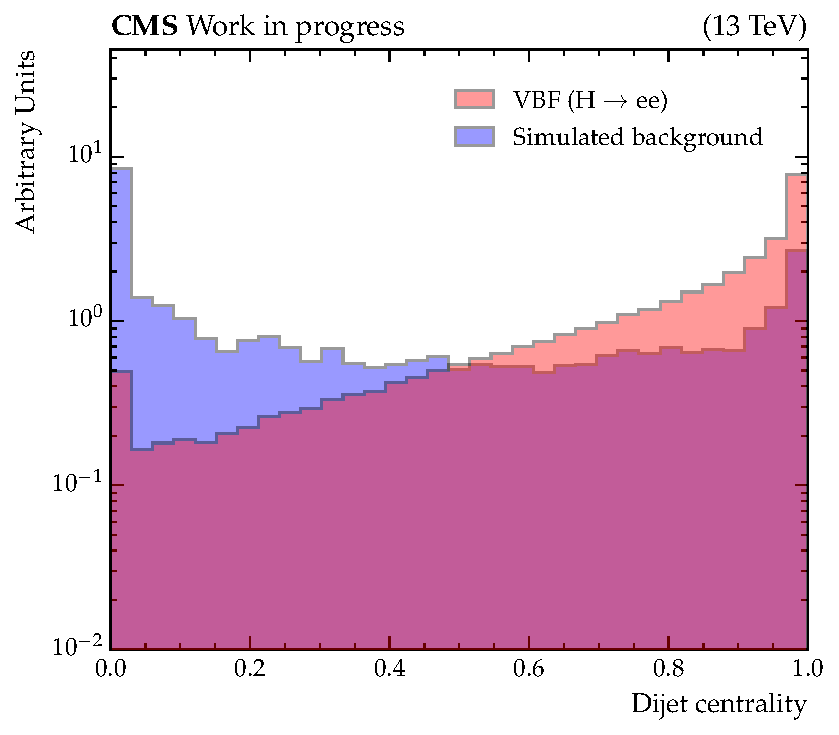
\includegraphics[width =0.45\linewidth]{Figures/Hee/VBF/normed/VBF_BDT_dijetCentrality_normalised.pdf}\hfill%

\caption[Distributions of selected input variables to the VBF BDT.]{The distributions for selected input variables to the VBF BDT. From top to bottom row, these include the magnitude of the difference in $\eta$ position between the leading two jets, the invariant mass of the system defined by the leading and subleading jets, and the centrality variable defined by the $\eta$ positions of the two leading jets and dielectron system. Left: feature distributions for simulated background processes (bold face), stacked for comparison with data (black points). Simulated VBF signal is also shown (red histogram), with the overall normalisation scaled such that it is visible. Reasonable agreement is observed between data and simulation, with respect to the statistical uncertainty (grey band). Right: the same input variables, normalised to unit area, with VBF signal shown in red, and simulated background integrated over each processes shown in blue. In general, the set of VBF input features display good separation between signal and background events.}
\label{fig:vbf_inputs}                                 
\end{figure}   


\subsection{Training and optimisation}

The training and optimisation procedure for the VBF BDT is identical to the \ggH BDT and hence will not be repeated in detail. The main hyperparameters of the model are optimised through a 3-fold cross-validation, with approximately ten thousand possible combinations considered. Simulated signal samples are reweighted by 1/$\sigma(\mee)$ to encourage high resolution events to occupy signal-like BDT scores. Finally, the sum of signal and background event weights are equalised during training in order to mitigate the large class imbalance.

\subsection{Performance evaluation}

Similarly to the \ggH BDT, the performance of the VBF BDT is evaluated using the area under the ROC curve. This metric is computed on both the training and testing sets, and compared as an overtraining check.
The output score of the VBF BDT used to construct the ROC curve is shown for simulated VBF signal, background, and data events in Figure~\ref{fig:vbf_out_score_and_rocs} (left). Unlike the \ggH BDT output score distribution, good separation between the signal and background classes is observed. In general, the classifier is able to reject DY and \ttbar events, which comprise the majority of the background yield, with high efficiency. Conversely, background events resulting from electroweak $\mathrm{Z}$ boson production, which exhibit signal-like topology, are harder to discriminate. These events account for up to 20\% of the total background in the most signal-like VBF BDT score bins.
The ROC curves for the training and testing sets are shown in Figure~\ref{fig:vbf_out_score_and_rocs} (right), with corresponding AUC values of 0.928 and 0.925 respectively.

\begin{figure}[htbp!]
\centering
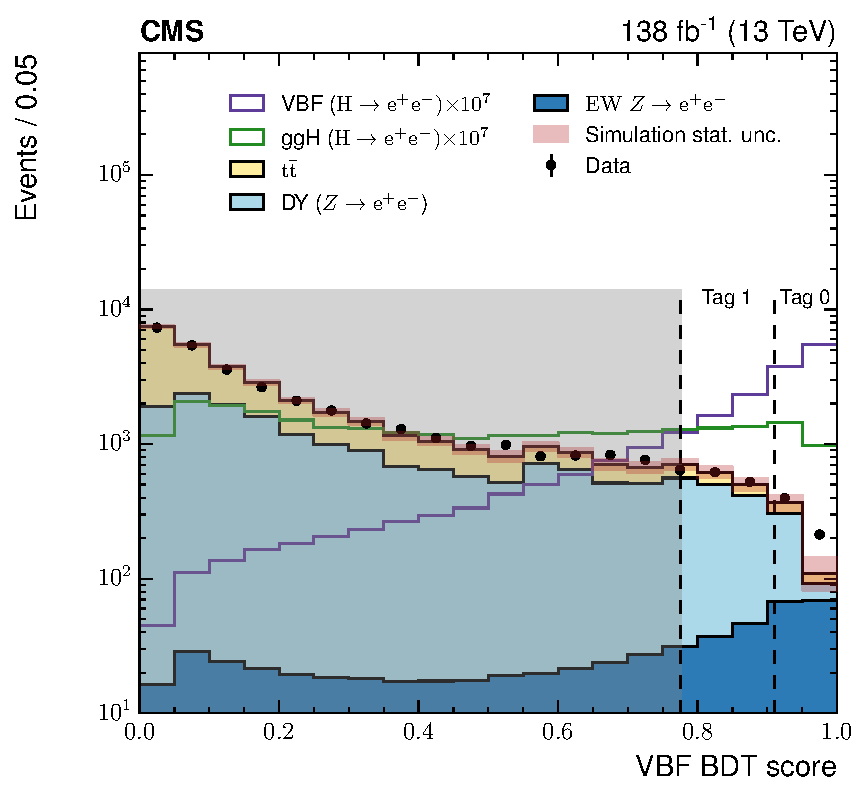
\includegraphics[width =0.485\linewidth]{Figures/Hee/VBF/dataMC/VBF_BDT_output_score_paper.pdf}\hfill%
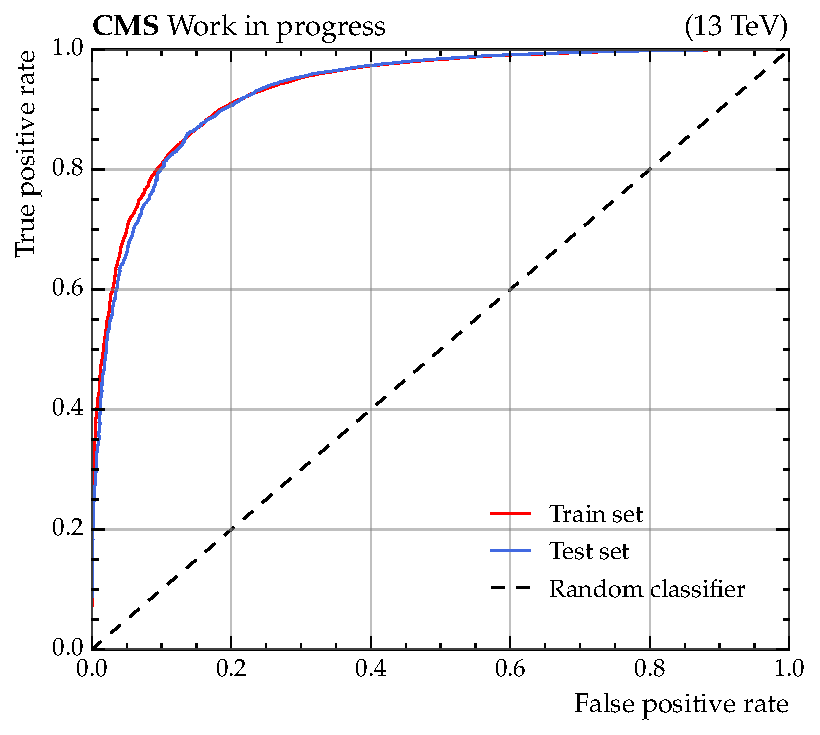
\includegraphics[width =0.5\linewidth]{Figures/Hee/VBF/dataMC/VBF_BDT_ROC_curve.pdf}\hfill%                           
\caption[The output score of the VBF BDT and associated ROC curve.]{Left: the output score of the VBF BDT in simulated signal events (green and purple histograms), background (bold face), and data (black markers) events. Good separation between the signal, and Drell-Yan and \ttbar backgrounds is observed. Category boundaries targeting VBF production are denoted with dashed lines. Events with scores in the low $S/B$ grey shaded region are not considered for VBF categories, but may populate categories targeting \ggH production. Right: receiver operating characteristic curves for the VBF BDT, evaluated separately on the training and testing datasets, with only VBF events considered as signal. The area under the curves, which measure classifier performance, are comparable for both sets indicating negligible overtraining. The dashed line (black) provides a benchmark for a model that assigns events to classes at random.}
\label{fig:vbf_out_score_and_rocs}
\end{figure}

\subsection{Model interpretation}

As discussed in Section \ref{subsec:ggh_categorisation}, for any complex classifier architecture, it is useful to investigate how the feature set is connected with the output predictions.
To understand how the inputs to the VBF BDT are correlated with the output score distribution, Figure~\ref{fig:vbf_feature_evo} shows a selection of the most predictive input features as a function of BDT score. Events associated with background-like predictions are shown in red and orange hues, while signal-like predictions comprising events predicted with high score are shown in green and blue. 
As expected, the VBF BDT assigns high scores to events characterised by a dijet pair with large invariant mass and angular separation of jets.
Also shown is the QGL ID value for the leading jet, which is expected a priori to hold reasonable rejection power against DY events, where jets are typically produced via radiated gluons. This is confirmed in Figure~\ref{fig:vbf_feature_evo}, where lower QGL scores are associated with background-like predictions.
Finally, similar distributions of the \mee spectrum in simulated signal and background events are produced to check both that the classifier assigns high scores to events with good mass resolution, and cannot learn the value of the Higgs boson mass.

\begin{figure}[htbp!] 
\centering 
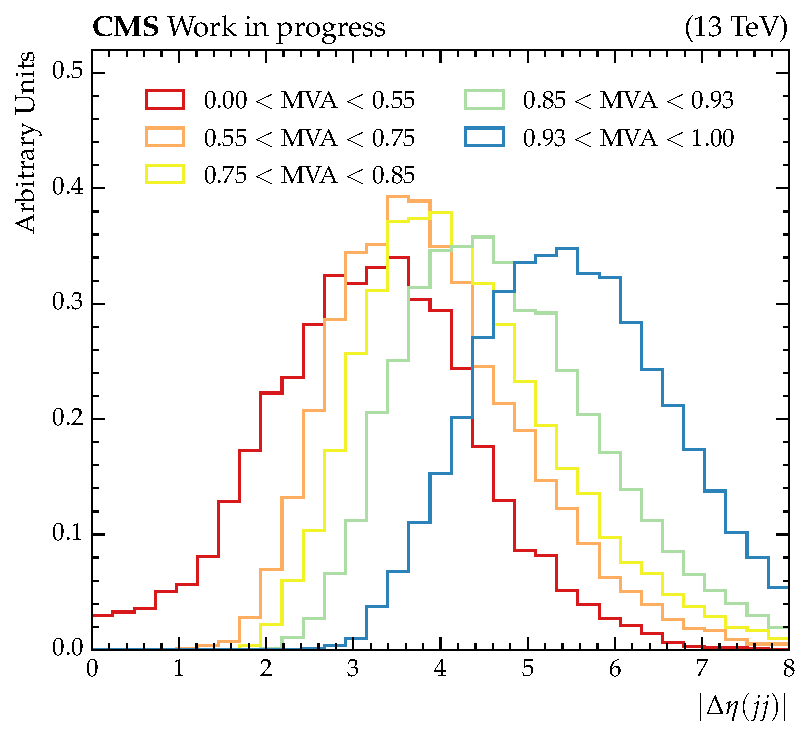
\includegraphics[width =0.325\linewidth]{Figures/Hee/VBF/featureEvo/VBF_BDT_dijetAbsDEta.pdf}
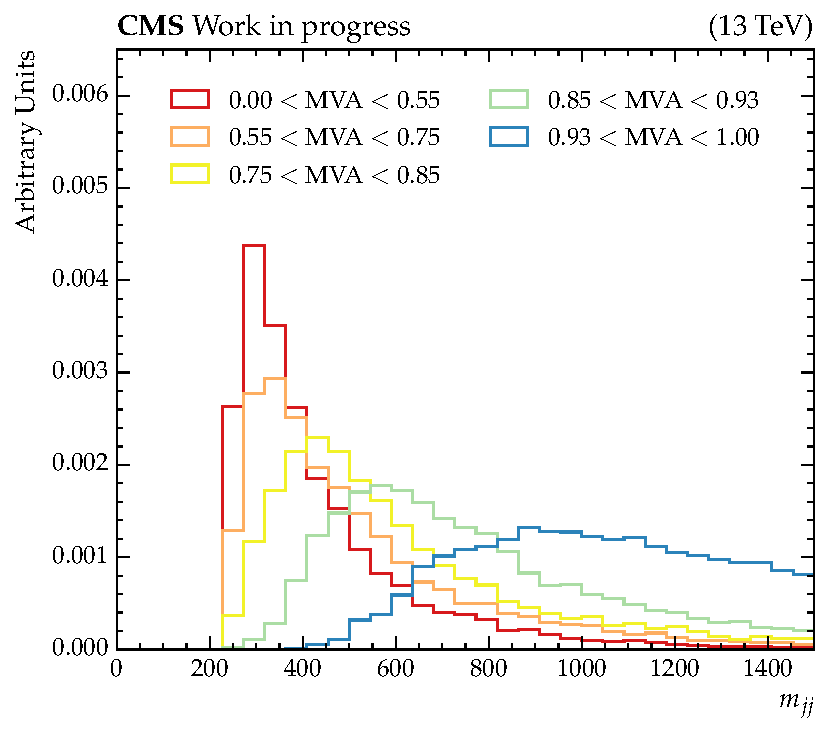
\includegraphics[width =0.334\linewidth]{Figures/Hee/VBF/featureEvo/VBF_BDT_dijetMass.pdf}\hfill
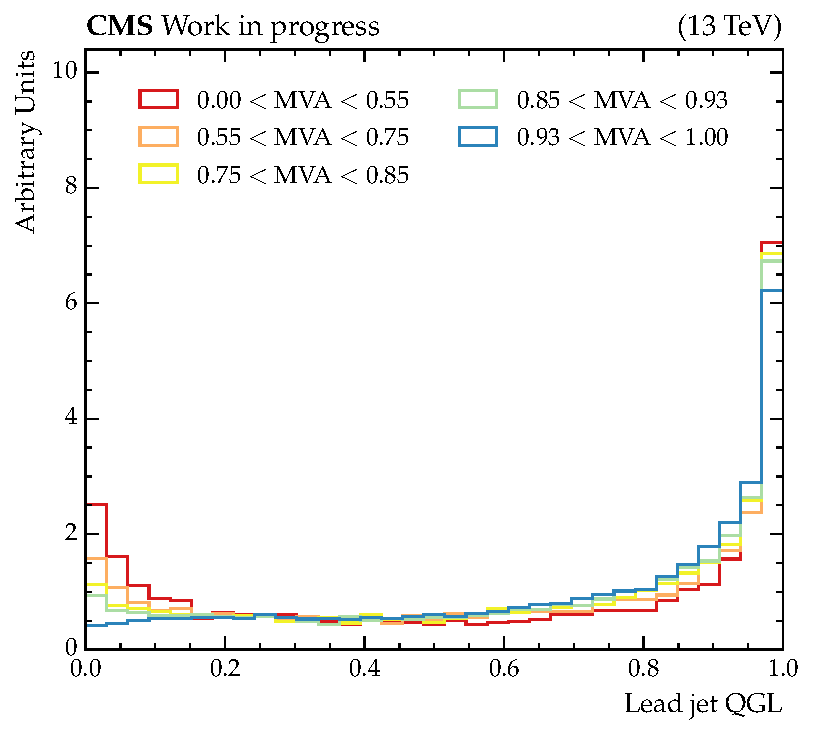
\includegraphics[width =0.325\linewidth]{Figures/Hee/VBF/featureEvo/VBF_BDT_leadJetQGL.pdf}\hfill

\caption[Distributions of selected inputs to the VBF BDT as a function of BDT output score.]{The distribution of selected inputs to the VBF BDT as a function of the VBF BDT score, in simulated VBF signal events. From left to right, these include the magnitude of the difference in $\eta$ position between the two leading jets, the invariant mass of the system defined by the leading and subleading jets, and the QGL ID score of the leading jet. Events obtaining a signal-like prediction are drawn in blue and green colours, while background-like events are shown in red and orange. Events with high dijet mass and angular separation of the leading two jets are associated with higher scores. Background-like scores are assigned to events with low (quark-like) QGL ID score.}
\label{fig:vbf_feature_evo}
\end{figure}

Similarly to the \ggH BDT, it is useful to generate Shapley values for the VBF BDT input feature set to understand which are the most important. Figure~\ref{fig:vbf_mee_and_njet_evo} shows the distribution of Shapley values at the per-event level, for a selection of the most predictive inputs. Quantities that encode jet kinematics typically score highly, including the dijet centrality and other angular descriptions. The directional pulls for each feature are also intuitive --- for example, higher values of centrality are typically associated with positive, signal-like predictions, which is expected from the distributions shown in Figure~\ref{fig:vbf_inputs}.

\begin{figure}[htbp!] 
\centering 
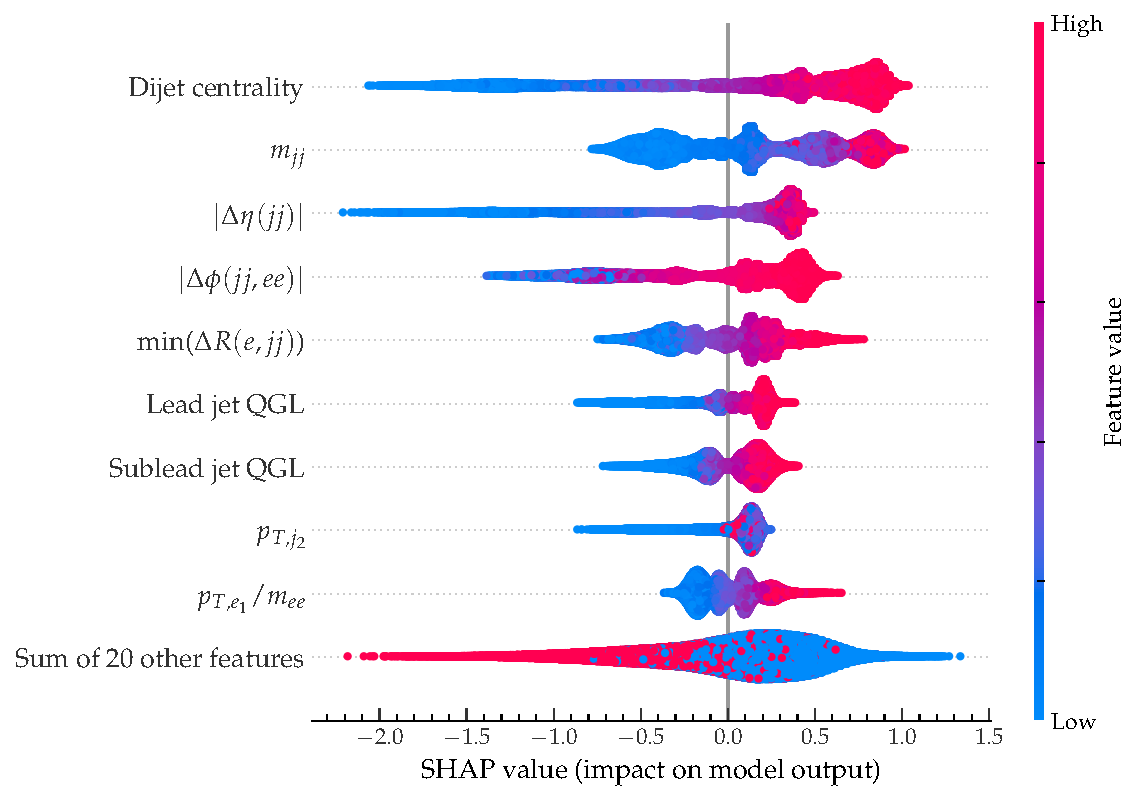
\includegraphics[width =0.8\linewidth]{Figures/Hee/VBF/featureImportances/shapley_beeswarm_VBF_BDT_featureSelection.pdf}
%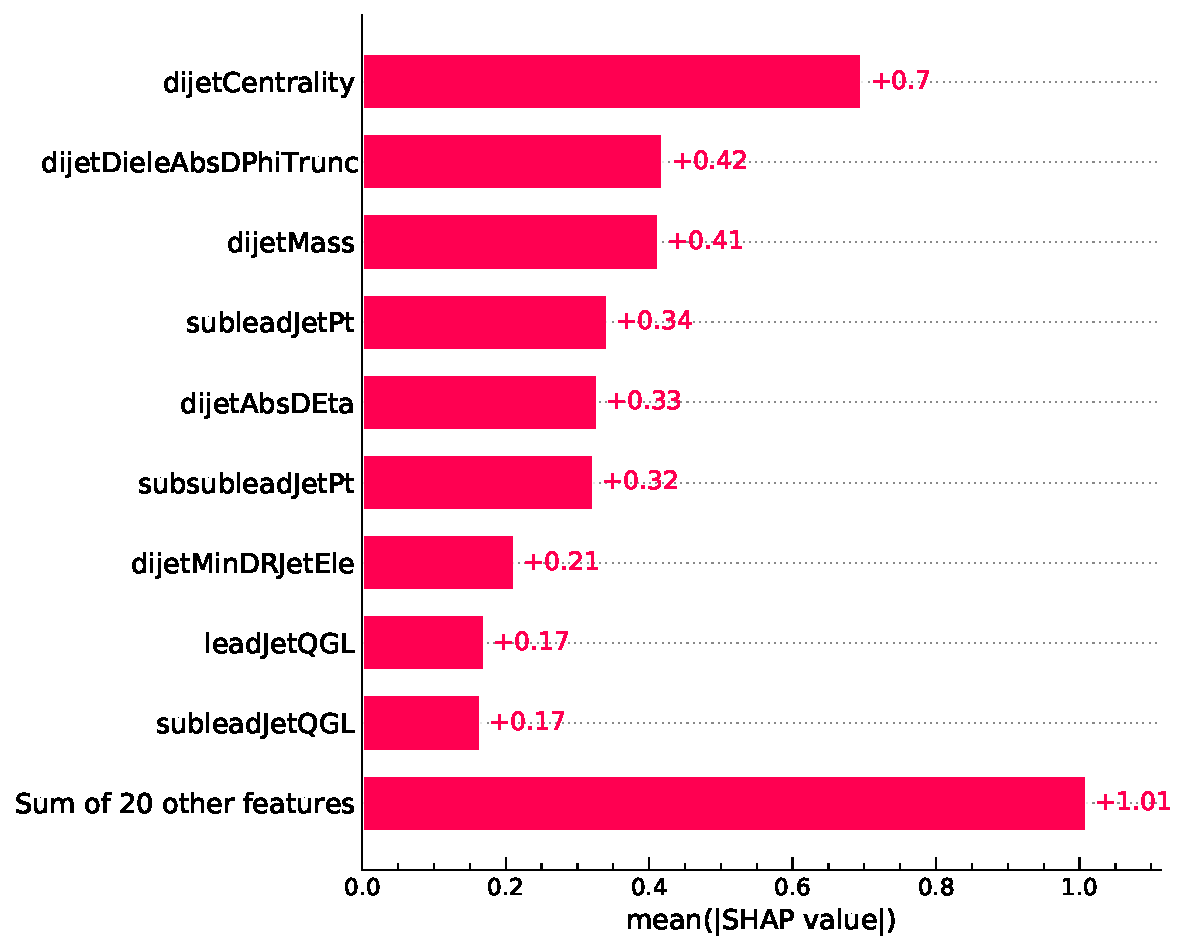
\includegraphics[width =0.8\linewidth]{Figures/Hee/VBF/featureImportances/shapley_bar_chart_VBF_BDT.pdf}
\caption[The feature importance for selected inputs to the VBF BDT.]{The distribution of Shapley values (filled circles) for selected input features to the VBF BDT, shown at the per-event level. Features are ordered by descending importance, measured by the mean of the absolute Shapley values over all events. Larger values of the input variable are coloured with red hues, while smaller values are shown in blue hues. The dijet centrality and invariant mass score highly, as expected from the large class separation visible in the 1D distributions. Events containing two jets separated by a large $\eta$ difference are also observed to pull the model output towards signal-like predictions, as expected.}
\label{fig:vbf_mee_and_njet_evo}
\end{figure}

\subsection{Category definitions}

To construct the final VBF categories, a boundary optimisation procedure identical to that presented in Section~\ref{subsec:ggh_categorisation} is followed, yielding two VBF categories. The resulting signal and background yields, fractional signal composition, and expected sensitivity are shown for each category in Table~\ref{tab:hee_s_b_ams}. The \mee distributions for simulated background events and data are shown for both VBF categories in Figure~\ref{fig:vbf_mee_dataMC}. In this phase space, the statistical uncertainty for simulated Drell-Yan events becomes large, partially motivating the data-driven method for constructing background models discussed in Section~\ref{subsec:hee_b_modelling}.

\begin{figure}[htbp!]
\centering
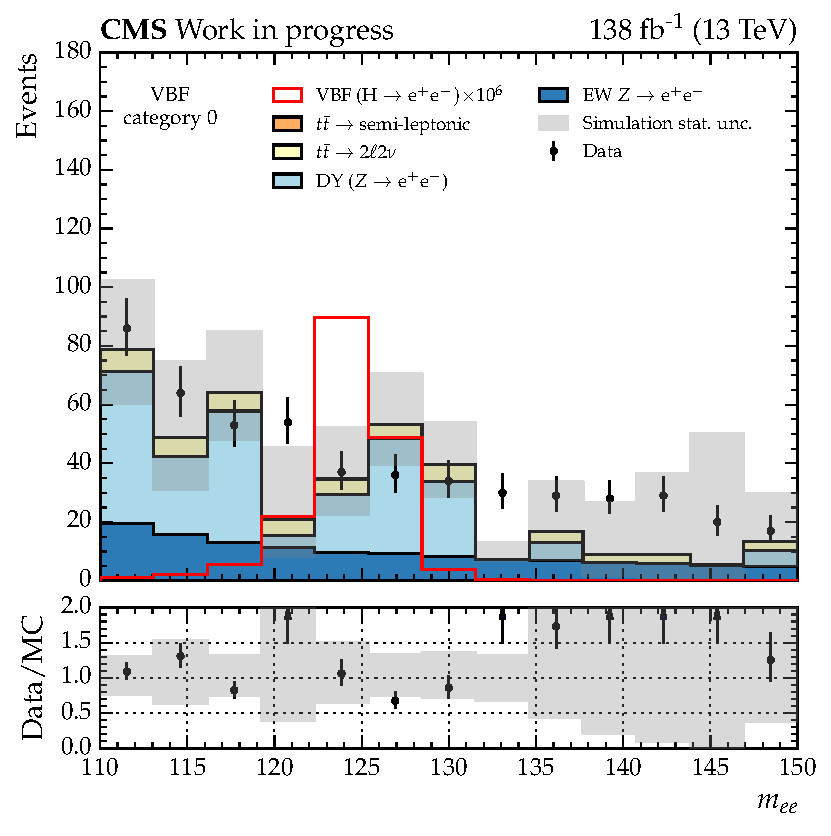
\includegraphics[width =0.48\linewidth]{Figures/Hee/VBF/MeePlots/VBF_BDT_dielectronMass_cat0.pdf}\hfill%
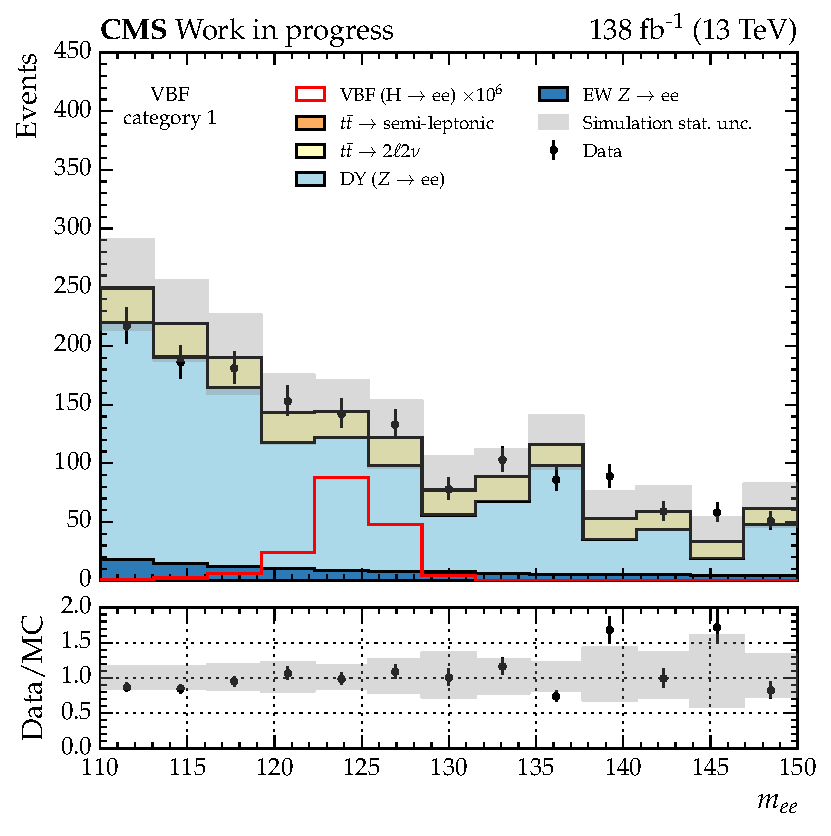
\includegraphics[width =0.48\linewidth]{Figures/Hee/VBF/MeePlots/VBF_BDT_dielectronMass_cat1.pdf}\hfill%
\caption[The dielectron mass distributions for analysis categories targeting VBF events.]{Observed \mee distributions for the two VBF analysis categories, shown for simulated background (bold face) and data (black points). The distribution for VBF signal events is also shown (red), with the overall yield scaled for visibility. The ratio of data to simulation is shown in the lower panel. Arrows indicate entries outside the $y$-axis range. The statistical uncertainty for DY events can be large for events with unphysically high simulated event weight, particularly in the higher $S/B$ analysis category.}
\label{fig:vbf_mee_dataMC}
\end{figure} 

\section{Deep learning based VBF categorisation strategies}
\label{subsec:vbf_lstm}

The BDT-based approach to background rejection in VBF categories makes use of features that are carefully engineered such that the distributions of signal and background events show
some separation power. However, in the process of summarising event information ``by hand", some of the original information in the event can be lost. This lost information may still provide discrimination power for the classification task, yet a BDT is unable to exploit it.
Therefore, it could be beneficial to invoke a machine learning algorithm that can abstract its own feature representations from low-level inputs. A deep neural network is a natural choice, where feature engineering occurs automatically within 
the network's hidden layers.



\subsection{Motivation and strategy}

The motivation for a neural network in the context of background rejection in the VBF phase space is two-fold. Firstly, summarising low-level detector information into higher-level input features with known predictive power is more suited to decision tree algorithms, where obvious partitions can be made in the input feature space. In comparison, a NN builds abstractions and higher-level representations from low-level inputs automatically within hidden layers, which may be more complex and indeed more useful that the original set of features chosen by hand. %EXAMPLE COMBINING JETS eta's FROM SAM.
Secondly, the structure of the input feature set could be arranged to appeal to the inductive bias of the choice of NN architecture, potentially resulting in additional separation power. 
% For example the correlation between neighbouring pixels is something that a CNN "adds" to the set of total usable information
% i guess low level features also appeals to the inductive bias of the NN too since its structure has auto feature egineering

The chosen VBF NN structure can be divided into two components. The first comprises long short-term memory layers which take low-level event features as input. These include the four vector and QGL ID score for the leading three jets in the event. The four vectors for the electrons are not provided to prevent the network from learning the value of \mee. Since the LSTM structure motivates the organisation of these jets by some meaningful ordering, the jet descriptions are arranged into a 1D sequence by descending jet \pt. This treatment is partially motivated by the DeepJet~\cite{deepJet} architecture for jet flavour tagging, where an LSTM is used to process a sequence of particle flow candidates, ordered by impact parameter.

In addition, a set of high-level input features are added such that the network can learn correlations between the low-level physics objects and the rest of the event. 
These are identical to those described in Section~\ref{subsec:vbf_categorisation} (minus the low-level features) and include electron kinematics and high-level jet features.
With this treatment, the input features are deliberately identical between models, in order to compare the NN and nominal BDT approaches fairly. The high-level features are combined with the output of the LSTM network in a series of fully connected layers. The number of nodes in each of these FC layers is designed to gradually reduce the dimensionality of the feature representations, before reaching the single output node. Hence, earlier FC layers are more dense than the latter ones. A summary of the architecture is illustrated in Figure \ref{fig:hee_VBF_lstsm}. %The dual structure of the network is heavily influenced by the tt(H$\rightarrow{}\gamma\gamma$) couplings analysis \cite{tthCouplings}, where LSTM units interfaced with FC layers are used within a classifier aiming to enhance \ttH signal events over $\gamma\gamma$ + jets and \ttbar+ $\gamma\gamma$ background processes.

\begin{figure}[htbp!] 
\centering 
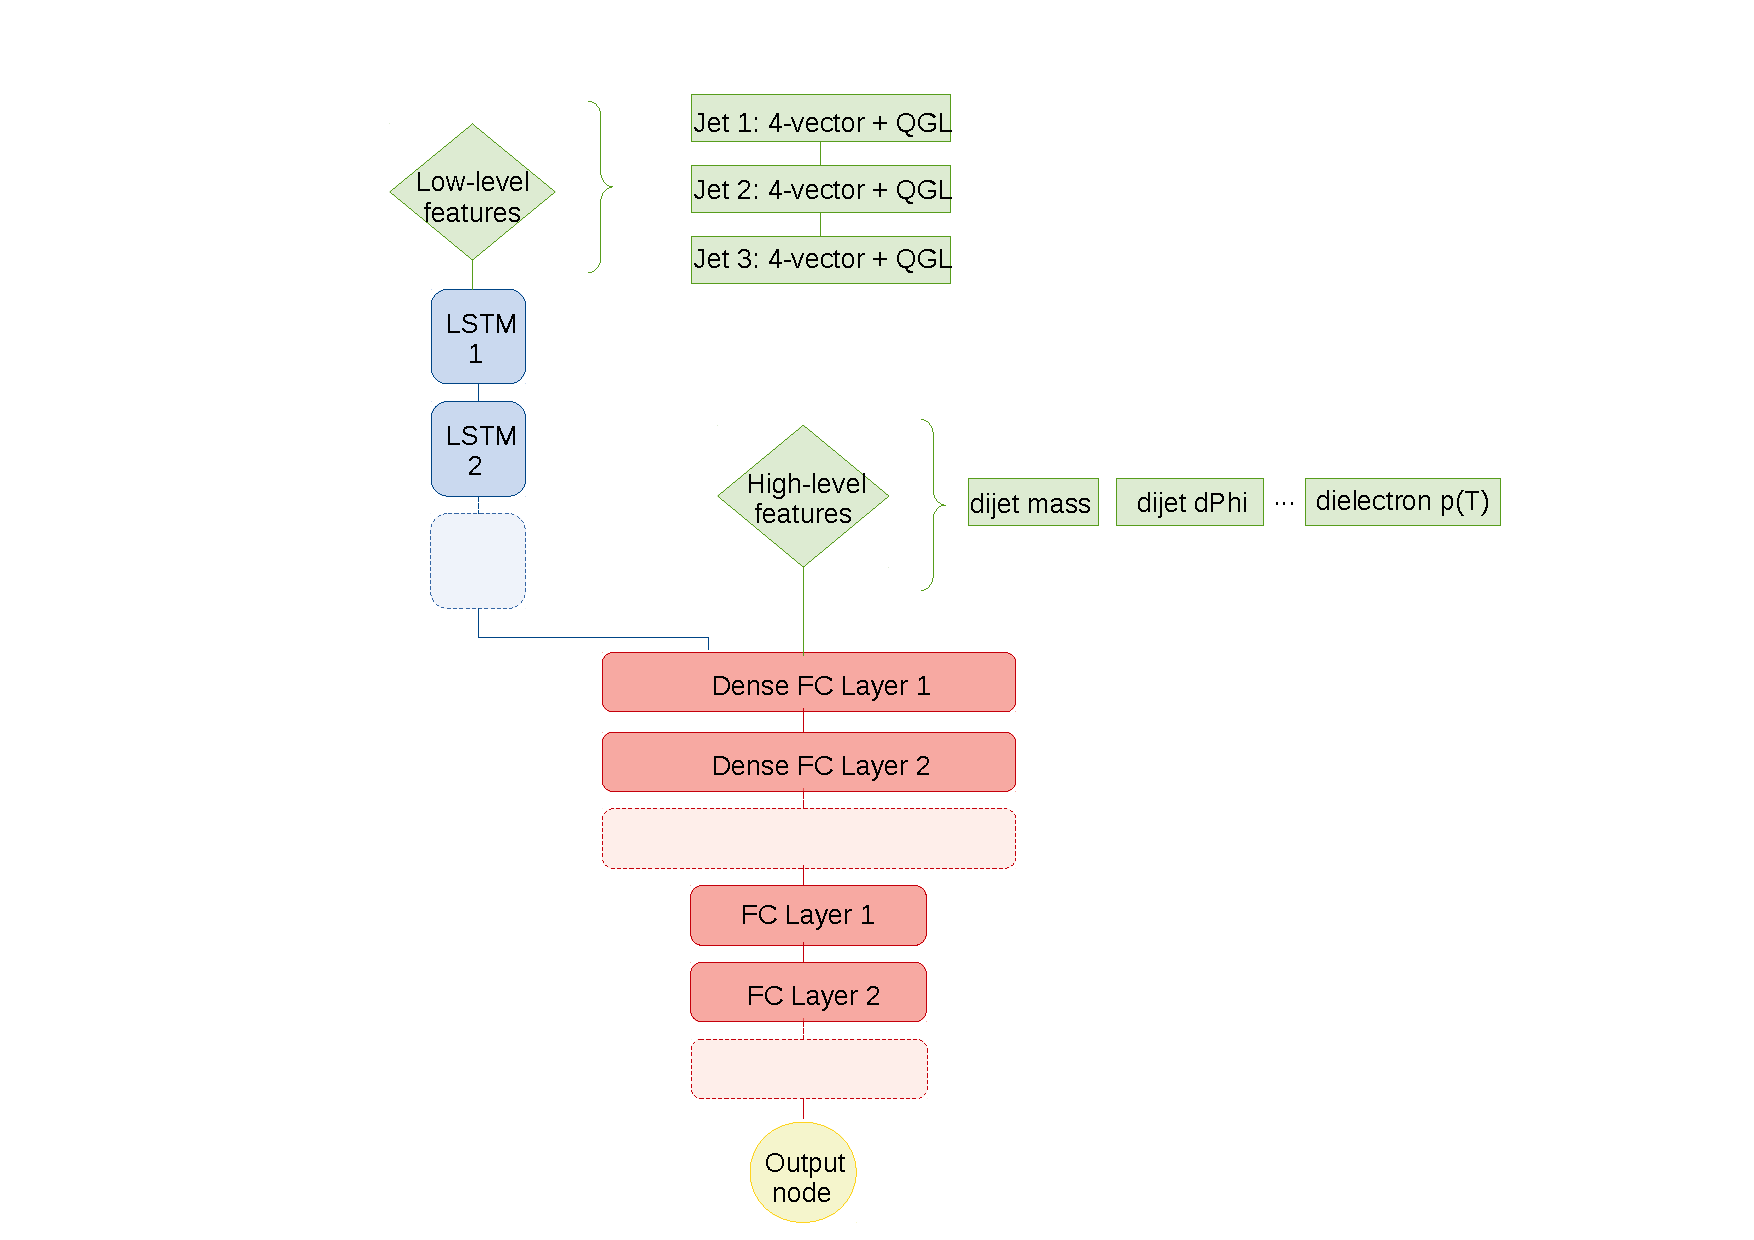
\includegraphics[trim={2cm 0cm 2cm 1cm},clip,width =1\linewidth]{Figures/Hee/VBF/DeepLearning/LSTM_general_structure.pdf}
\caption[The VBF LSTM neural network architecture.]{A schematic of the VBF neural network architecture. The structure comprises long short-term memory layers (blue) which take low-level descriptions of the three leading jets. The output from the final long short-term memory cell is interfaced with fully connected layers (red) which take high-level per-event features as inputs. The number of nodes in each layer is decreased gradually before reaching the terminal output node (yellow) which holds the discriminator score. Empty components indicate possible extensions to the network architecture that are explored during hyperparmeter tuning.}
\label{fig:hee_VBF_lstsm}
\end{figure}

\subsection{Training and optimisation}

The network is implemented using the \textsc{Keras}~\cite{keras} python library, with the \textsc{Tensorflow}~\cite{tensorflow} backend. The differentiable loss function for the categorisation task is chosen to be identical to the BDT-based approach, since the classification goal is identical. Although \textsc{Keras} supports many gradient-descent based algorithms to minimise this loss, in practise, the Adam~\cite{adam} optimiser is chosen. Adam uses an approach similar to classical SGD, with a variable learning rate that is gradually decreased as the number of steps taken by the optimiser increases. 

Several hyperparameters of the network are optimised as part of the model selection process.
For the LSTM portion of the network, the number of hidden layers and number of nodes
in each layer are optimised. A similar strategy is employed for the fully connected network layers. To regularise the network, a dropout technique is implemented~\cite{dropout}, where the exact probability to drop each neuron is considered as a hyperparameter. Each of the above network parameters are optimised using a grid search strategy, where a range of possible hyperparameter values are specified, and a model is trained for each possible combination. This results in the training of a few thousand networks. The final choice of NN hyperparameters that maximise the model performance is summarised in Table \ref{tab:dnn_final_hps}. Note, however, that the performance is largely insensitive to the exact hyperparameter choices; most configurations return equally performant models.
 
Input features are also pre-processed with a ``Z-score" normalisation procedure,
where the mean and standard deviation are transformed to be zero and one respectively. These transformations provide a uniform scale for all features, a common technique used to speed up convergence during training and improve network performance~\cite{backprop}.

Finally, to further prevent overfitting, the network is trained with an early-stopping procedure in which the number of training epochs is decided dynamically by the loss, computed on a validation set containing 20\% of the events. During this process, the batch size is also increased while training, to encourage convergence to the global minimum~\cite{batch_boost}. 
 
\begin{table}[htbp!]
\centering
\caption[The hyperparameter configuration for the VBF LSTM neural network.]{The optimal choice of hyperparameters for the VBF NN, chosen to maximise the network performance on a withheld validation set. A grid search strategy over the potential architecture space is performed, resulting in the training of a few thousand networks. Multiple entries indicate the configuration for successive units of the same type.}
\label{tab:dnn_final_hps}
\begin{tabular}{l|l}
\hline
Network hyperparameter    & Value(s) \\ \hline 
Number of FC layers & 3       \\
Number of nodes in each FC layer & 200, 100, 100\\
Number of LSTM layers & 2 \\
Number of nodes in each LSTM layer & 100, 100 \\
Dropout rate & 0.2 \\ 
Activation function (FC layers) & Rectified linear unit \\
Activation function (output layer) & Sigmoid \\
\hline
\end{tabular}                  
\end{table}  


\subsection{Performance comparisons}

The performance of the VBF NN is compared with the nominal BDT-based approach to assess whether the deep learning architecture offers any improvement in background rejection. The figure of merit in this comparison is the area under the ROC curve for each model, which for the VBF NN is generated from the output score distribution shown in Figure~\ref{fig:vbf_nn_vs_bdt} (left). The distribution of scores is similar between the VBF NN and nominal VBF BDT (Figure~\ref{fig:vbf_out_score_and_rocs}); the simulated signal is well separated from both the DY and \ttbar backgrounds, while backgrounds from EW $\mathrm{Z}$ processes are harder to separate. The areas under the corresponding ROC curves, shown in Figure~\ref{fig:vbf_nn_vs_bdt} (right), are also similar between classifiers --- when evaluated on the test set, the area under the ROC curve associated with the VBF NN (BDT) is 0.923 (0.925). It is therefore concluded that, for this learning task, a more complex approach using a deep learning-based classifier offers near identical performance to the nominal BDT-based approach. %ReLu is good for vanishing gradients; note that a gradient of zero wouldn't be a problem, if we could get it non-zero again in later epochs (but we can't vey easily!). Because lets say the gradient ap epoch 2 is zero somewhere, and we realise that didn't the best weight update in the next step, we would want to make it non-zero, but now we can't because that section of the network is dead.

\begin{figure}[htbp!]
\centering
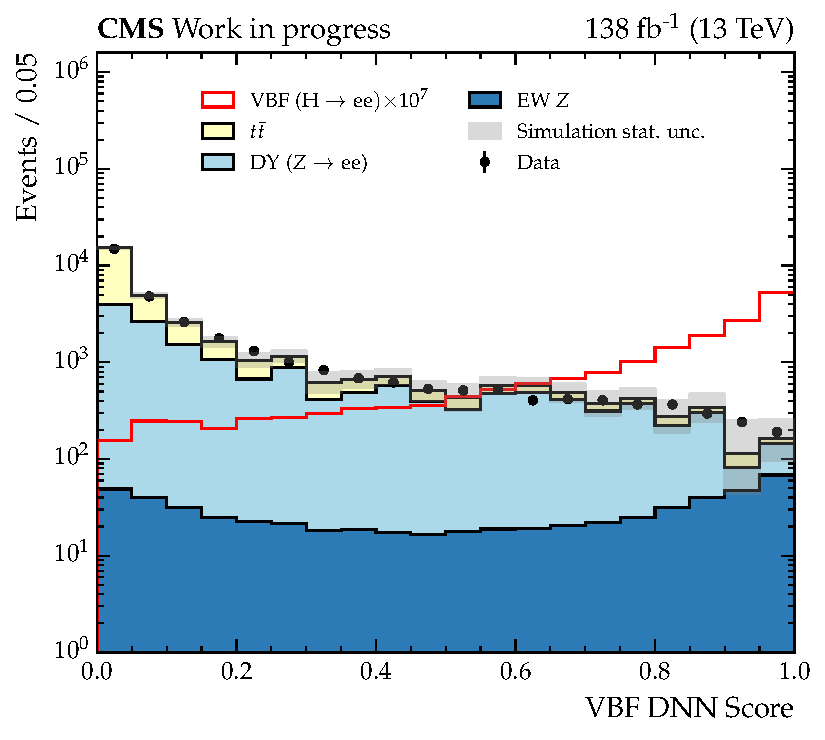
\includegraphics[width =0.5\linewidth]{Figures/Hee/VBF/DeepLearning/performanceComparison/VBF_DNN_output_score.pdf}\hfill%
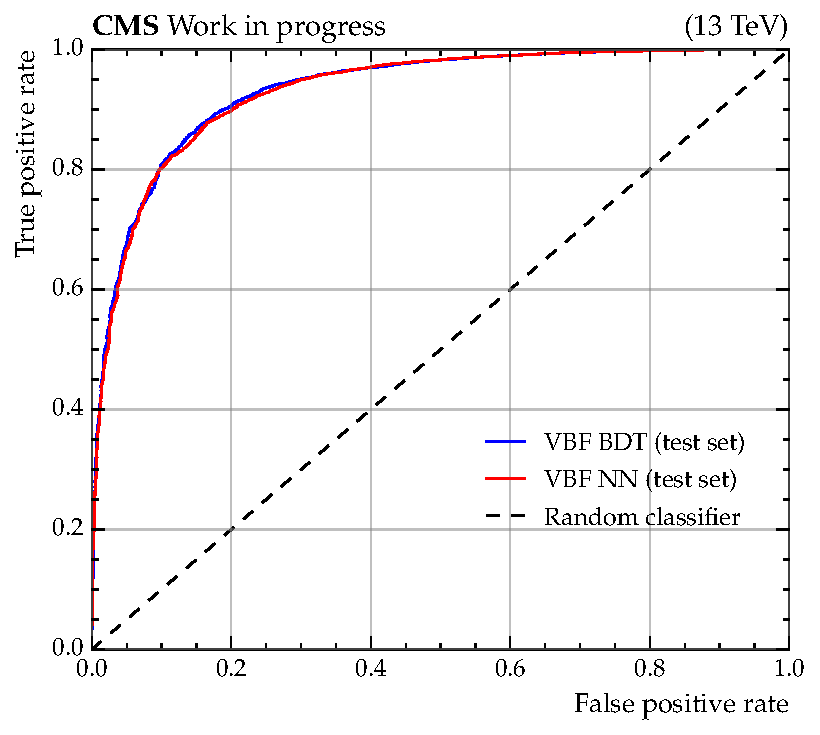
\includegraphics[width =0.5\linewidth]{Figures/Hee/VBF/DeepLearning/performanceComparison/VBF_BDT_vs_DNN_ROC.pdf}\hfill%                           
\caption[The output score of the VBF LSTM neural network.]{Left: the output score of the VBF NN in simulated signal (red), background (bold face), and data (black markers). The separation observed between the signal, and Drell-Yan and \ttbar backgrounds is similar to that of the VBF BDT. Right: ROC curves for the VBF NN (red) and the VBF BDT (blue), evaluated on the test set. The area under the curves are comparable between models, indicating similar performance.}
\label{fig:vbf_nn_vs_bdt}
\end{figure}

To understand why the two learning algorithms may perform similarly, it is again useful to understand how the model predictions are connected with the input features. To this end, a selection of the most predictive features are shown as a function of the VBF NN output score in Figure~\ref{fig:vbf_feature_evo_dnn}. The evolution of each feature is almost identical to the analogous distributions for the VBF BDT shown in Figure~\ref{fig:vbf_feature_evo}, suggesting that input features are being used in similar ways. Both models assign high scores to events containing a dijet pair with high invariant mass, and large separation in pseudorapidity between the constituent jets. The fact that both algorithms produce models yielding similar performances, using variables in near identical ways, suggests that the underlying function mapping input features to the target class is learned near optimally. This is also supported by the fact that the NN performance is largely insensitive to the exact choice of architecture during hyperparameter optimisation; each model returns a similar performance, regardless of its complexity.


\begin{figure}[htbp!] 
\centering 
\includegraphics[width =0.32\linewidth]{Figures/Hee/VBF/DeepLearning/interpretation/VBF_DNN_dijetAbsDEta.pdf}
\includegraphics[width =0.32\linewidth]{Figures/Hee/VBF/DeepLearning/interpretation/VBF_DNN_dijetMass.pdf}\hfill
\includegraphics[width =0.33\linewidth]{Figures/Hee/VBF/DeepLearning/interpretation/VBF_DNN_leadJetQGL.pdf}\hfill

\caption[The distribution of selected inputs to the VBF LSTM neural network as a function of the model output score.]{Distributions of selected inputs to the VBF NN as a function of VBF NN output score, in simulated VBF signal events. Each histogram is normalised to unit area. The variables shown have identical definitions to those in Figure~\ref{fig:vbf_feature_evo}. The evolution of each feature with the NN score is almost identical to the analogous plots for the VBF BDT, suggesting that variables are used in similar ways between the two classifier types.}
\label{fig:vbf_feature_evo_dnn}
\end{figure}

%In addition, the representing low-level input features as a sequence with an abstract ordering by \pt, within an LSTM architecture, 
An alternative explanation is that the representation of features, combined with the choice of learning algorithm, may not offer any additional information for the task. Although ordering low-level jet inputs by \pt has been shown to offer small improvements in other applications~\cite{tthCouplings}, LSTM input data is typically ordered temporally. This is perhaps a more natural ordering, where the connection between elements is less abstract and can be easily interpreted by the model. In the case of the VBF classification task, an alternative structuring of the input dataset may appeal more naturally to the inductive bias of alternative algorithms. For example, treating the jet-based information as an image, unfolded in the $\eta$-$\phi$ detector plane, and applying a convolutional NN has been shown to offer a small advantage over BDT-based approaches for VBF classification in the \Hgg decay channel~\cite{jack_thesis}. 

Given the similarity between performances, the nominal VBF BDT-based approach is kept for VBF classification. This model is significantly quicker to train and uses less computational resources than the deep learning approach.


\section{BDT validation}

In this analysis, background models are taken directly from data, whereas signal models are derived from simulated samples. Therefore, it is necessary to ensure there is reasonable agreement between data and simulation for signal-like objects in the inputs to each BDT, which in turn control agreement in the output score. 
This is validated using a sample of \Zee events from control regions in data, defined to be orthogonal to the analysis category phase space. Drell-Yan processes are chosen for this validation since a large number of events that mimic the \Hee final state are available, and the decay is relatively free from contaminating backgrounds. For the \ggH BDT, the control region is defined by the nominal analysis preselection, with the exception of the dielectron mass requirements which are shifted to 80 $<$ \mee $<$ 100~GeV, in order to roughly centre on the $\mathrm{Z}$ boson mass.
For validation of the VBF BDT, the VBF preselection defined in Section~\ref{subsec:vbf_categorisation} is applied in addition.

Figure~\ref{fig:hee_ggh_vbf_validation} shows the output score distribution of both the \ggH and VBF BDT for data and simulation. 
The effect of the dominant systematic uncertainties are included in both plots. For electrons, these include the uncertainty on the electron energy scale corrections, and uncertainties on the electron reconstruction and identification efficiencies. For inputs that describe jets, the uncertainties associated with the jet energy scale and resolution corrections are also included. The agreement between data and simulation in both output score distributions is within the uncertainty permitted by the combined systematic and statistical variations, over the majority of each distribution. The residual differences observed in the \ggH BDT score are smaller than the \ggH theoretical uncertainties included in the final fits, presented in Section~\ref{subsec:hee_syst_uncertainties}. The closure between data and simulation for the input features to both BDTs is also good. 

\begin{figure}[htbp!]
\centering
\includegraphics[width=0.49\textwidth]{Figures/Hee/ggH/validation/DY_validation_ggH_BDT_ggH_mva_paper.pdf}\hfill%
\includegraphics[width=0.49\textwidth]{Figures/Hee/VBF/validation/DY_validation_VBF_BDT_VBF_mva_paper.pdf}\hfill%
\caption[The output score distribution for the \ggH and VBF BDTs for \Zee events in the \Hee control region.]{Distribution of the output score of the ggH BDT (left) and VBF BDT (right) in their respective \Zee control regions. The combination of systematic and statistical uncertainties is shown by the red shaded band. Category boundaries targeting each Higgs boson production process are denoted with dashed lines. Events with scores in the low $S/B$ grey shaded regions are not considered for their respective categories. Good agreement is observed between the Drell-Yan simulation (filled histograms) and data (black points), for the phase space in which analysis categories are constructed.  For the ggH BDT output score, residual differences between the data and simulation are covered by theoretical uncertainties on the \ggH cross section included in the final fits.}% The overall magnitude of this uncertainty is shown explicitly in the shaded blue band}
\label{fig:hee_ggh_vbf_validation}
\end{figure}

\section{Summary}
\label{hee_categorisation_summary}

The categorisation for \Hee events targets production via both gluon fusion and vector boson fusion. Analysis categories are constructed using the output of dedicated BDTs, designed to improve the $S/B$ ratio. Each BDT is trained on kinematic properties of the dielectron object, alongside descriptions of any associated jets. For the categorisation of VBF events, a deep learning approach using a long short-term memory neural network is also studied, yielding similar performance to the nominal BDT-based approach. Two categories are developed to target VBF events, while four categories are used for \ggH. Events satisfying requirements for both VBF and \ggH categories are assigned preferentially to those targeting VBF, as illustrated in Figure~\ref{fig:hee_tag_sequence}.

\begin{figure}[htbp!]
\centering
\includegraphics[trim={0cm 0cm 7cm 7cm}, clip, width=0.9\textwidth]{Figures/Hee/Misc/tagSequence.pdf}\hfill%
\caption[The priority sequence for categorisation of \Hee events.]{The priority sequence for \Hee analysis categories. Events are considered firstly for one of two categories targeting VBF, provided they pass the jet-based VBF preselection. Events failing the VBF preselection requirements, or receiving VBF BDT scores lower than the minimum category BDT threshold, are then considered for one of four \ggH categories. Events that do not satisfy the requirements for any category, or that do not pass the analysis preselection (equivalent to the \ggH selection), are discarded.}
\label{fig:hee_tag_sequence}
\end{figure}